\section{SIMULA}
\label{sec:SIMULA}

Como suporte às operações relacionadas à manipulação de dados georreferenciados relativos aos ambientes de simulação utiliza-se um \textit{software} especificamente desenvolvido para tal função, denominado SIMULA. Ele desempenha as funções de aquisição, tratamento e disponibilização de informações georreferenciadas ao programa que executa as simulações e ao módulo visualizador de saídas, sendo um \textit{software} que integra operações de pré-processamento, como aquisição e tratamento de dados e de pós-processamento, como a visualização de saídas gráficas de arquivos resultantes das simulações executadas. 

Na etapa de aquisição dos dados o \textit{software} realiza consultas em um Sistema Gerenciador de Banco de Dados Objeto Relacional, SGBDOR, utilizando a linguagem de consulta \textit{Structured Query Language}, SQL. Nesta etapa são obtidas informações sobre os pontos georreferenciados dos polígonos que representam os lotes e ruas do ambiente. Foi utilizado o SGBDOR PostgreSQL com a adição da extensão PostGIS, que viabiliza o armazenamento e processamento de objetos com informações georreferenciadas em bancos de dados. Por meio da extensão PostGIS os dados são importados para o banco de dados a partir de um arquivo em formato \textit{shapefile}, que é um formato de arquivos utilizado para o armazenamento de dados geoespaciais. Os arquivos \textit{shapefile} utilizados neste trabalho foram obtidos em parceria com a prefeitura da cidade de Cascavel/PR. 

Na próxima sub-seção são apresentadas as funções SQL utilizadas para obtenção das informações necessárias à representação computacional do ambiente em simulação, com o objetivo de viabilizar a execução das operações definidas na Seção \ref{sec:estruturasDadosEstrategiasImplementacao}. Por manipular grandes quantidades de dados as funções apresentadas possuem alto tempo de execução. Considerando este fato e objetivando reduzir os tempos de computação para obtenção das informações necessárias, as funções somente são executadas quando há alteração na tabela de polígonos do ambiente. Quando executadas seus resultados são armazenados em tabelas auxiliares que viabilizam a rápida recuperação dos dados. Desde modo o banco de dados armazena todas as informações pré-computadas referentes à representação do ambiente e de outras informações pertinentes. 

\newpage

\subsection{Operações Executadas no Banco de Dados}

O Código \ref{cod:sql_consultasPrincipais} ilustra as principais operações realizadas no banco, que incluem a remoção e criação de tabelas e alteração do refinamento relacionado ao ambiente. A função de remoção de tabelas exclui as tabelas auxiliares relacionadas ao ambiente, sendo executada quando necessário atualizar as tabelas auxiliares devido à alguma mudança nos dados. A função de criação de tabelas cria as tabelas auxiliares no banco de dados. Por fim a consulta de alteração de refinamentos altera o refinamento de um determinado ambiente. O nome do ambiente alvo das funções é passado como argumento.

\lstinputlisting[caption=Consultas principais realizadas no banco de dados, label=cod:sql_consultasPrincipais, captionpos=b, language=SQL]{Codigos/Simula/Consultas/consultasPrincipais.sql}

\subsubsection{SQL de Criação das Tabelas}

O Código \ref{cod:sql_criarTabelas} ilustra a função de criação das tabelas auxiliares. São criadas durante a execução desta função três tabelas auxiliares, que armazenam diferentes informações relevantes à representação do ambiente. As informações utilizadas à criação de cada tabela são obtidas por funções distintas que são chamadas por esta função. Estas funções são apresentadas nos Códigos \ref{cod:sql_criarTabelaPontos}, \ref{cod:sql_getVizinhancasEntrePoligonos} e \ref{cod:sql_getVizinhancasMoorePontos}.

\lstinputlisting[caption=Função criarTabelas, label=cod:sql_criarTabelas, captionpos=b, language=SQL]{Codigos/Simula/Consultas/criarTabelas.sql}

\subsubsection{SQL de Remoção das Tabelas}

O Código \ref{cod:sql_removerTabelas} ilustra a função de remoção das tabelas auxiliares. São removidas as tabelas que possuam como prefixo o nome do ambiente passado à função. 

\lstinputlisting[caption=Função removerTabelas, label=cod:sql_removerTabelas, captionpos=b, language=SQL]{Codigos/Simula/Consultas/removerTabelas.sql}

\subsubsection{SQL de Interpolação de Pontos}

O Código \ref{cod:sql_interpolarPontos} ilustra a função de interpolação de pontos utilizando o método de interpolação linear. Esta função interpola pontos equiespaçados internos à um polígono, sendo o polígono e a distância de espaçamento entre os pontos passados como argumentos à função. Esta função é utilizada pela função de criação da tabela de pontos, apresentada no Código \ref{cod:sql_criarTabelaPontos}. 

\lstinputlisting[caption=Função interpolarPontos, label=cod:sql_interpolarPontos, captionpos=b, language=SQL]{Codigos/Simula/Consultas/interpolarPontos.sql}

\subsubsection{SQL de Criação da Tabela de Pontos}

O Código \ref{cod:sql_criarTabelaPontos} ilustra a função de criação da tabela de pontos que utiliza a função apresentada no Código \ref{cod:sql_interpolarPontos}. A interpolação dos pontos é realizada independentemente para cada lote pertencente ao ambiente passado como argumento à função. A execução desta função resulta na criação de uma tabela com o nome do ambiente e o sufixo \textit{"\_pontos"}. A Tabela \ref{tab:cascavel_pontos} ilustra as dez primeiras linhas dos dados gerados por esta função para o ambiente de Cascavel/PR. A coluna de geometria foi omitida por conter informações não interpretáveis.

\lstinputlisting[caption=Função criarTabelaPontos, label=cod:sql_criarTabelaPontos, captionpos=b, language=SQL]{Codigos/Simula/Consultas/criarTabelaPontos.sql}

\begin{table}[H]
\centering
\pgfplotstabletypeset[
col sep = semicolon,
every head row/.style={before row=\toprule,after row=\midrule},
every last row/.style={after row=\bottomrule},
string type
]{Figuras/Simula/Tabelas/cascavel_pontos.csv}
\caption{Tabela cascavel\_pontos.}
\label{tab:cascavel_pontos}
\end{table}

\subsubsection{SQL de Criação da Tabela de Vizinhanças entre Polígonos}

O Código \ref{cod:sql_getVizinhancasEntrePoligonos} ilustra a função de criação da tabela que armazena as vizinhanças entre polígonos. Nesta tabela são descritas as vizinhanças entre polígonos que representam os lotes e as ruas. Esta descrição das vizinhanças entre polígonos são obtidas utilizando a função \textit{st\_dwithin} da extensão PostGIS. A função \textit{st\_dwithin} retorna verdadeiro caso as duas geometrias passadas como argumento estão a uma distância menor ou igual à distância também passada como argumento. A tabela resultante desta função é nomeada pelo ambiente e o sufixo \textit{"\_vizinhancasentrepoligonos"}. A Tabela \ref{tab:cascavel_vizinhancasentrepoligonos} ilustra as dez primeiras linhas dos dados gerados por esta função para o ambiente de Cascavel/PR.

\lstinputlisting[caption=Função getVizinhancasEntrePoligonos, label=cod:sql_getVizinhancasEntrePoligonos, captionpos=b, language=SQL]{Codigos/Simula/Consultas/getVizinhancasEntrePoligonos.sql}

\begin{table}[H]
\centering
\pgfplotstabletypeset[
col sep = semicolon,
every head row/.style={before row=\toprule,after row=\midrule},
every last row/.style={after row=\bottomrule},
string type
]{Figuras/Simula/Tabelas/cascavel_vizinhancasentrepoligonos.csv}
\caption{Tabela cascavel\_vizinhancasentrepoligonos.}
\label{tab:cascavel_vizinhancasentrepoligonos}
\end{table}

\subsubsection{SQL de Criação da Tabela de Vizinhanças de Moore entre Pontos}

O Código \ref{cod:sql_getVizinhancasMoorePontos} ilustra a função de criação da tabela que armazena as vizinhanças de Moore entre os pontos. Estas vizinhanças têm papel importante durante a execução das simulações, pois definem as relações de conectividade utilizadas na movimentação de agentes. O desempenho computacional desta função é altamente dependente dos refinamentos escolhidos, pois quanto menor o refinamento, maior serão as quantidades de pontos gerados e de vizinhanças calculadas. Para obter os vizinhos de um ponto qualquer é utilizada a função \textit{st\_dwithin}, que verifica se dois pontos estão à uma distância menor ou igual à distância passada como argumento à função. A distância máxima considerada para a vizinhança de Moore é definida por $D_{max} = r_{max} * \sqrt{2} + 0.1$, em que $r_{max}$ designa o máximo dos refinamentos entre os dois pontos. Para acelerar o processo de obtenção das vizinhanças, o espaço de buscas é restrito aos próprios pontos do lote e aos pontos dos lotes vizinhos, utilizando as informações provenientes da tabela criada pelo Código \ref{cod:sql_getVizinhancasEntrePoligonos}. Desta forma, para o cálculo da vizinhança de Moore de um ponto qualquer $V$, a função \textit{st\_dwithin} somente é executada para os pontos que pertencem ao mesmo lote $l$ de $V$ ou aos lotes vizinhos de $l$. A tabela resultante desta função é nomeada pelo ambiente e o sufixo \textit{"\_vizinhancasmoorepontos"}. A Tabela \ref{tab:cascavel_vizinhancasmoorepontos} ilustra as dez primeiras linhas dos dados gerados por esta função para o ambiente de Cascavel/PR.

\lstinputlisting[caption=Função getVizinhancasMoorePontos, label=cod:sql_getVizinhancasMoorePontos, captionpos=b, language=SQL]{Codigos/Simula/Consultas/getVizinhancasMoorePontos.sql}

\begin{table}[H]
\centering
\pgfplotstabletypeset[
col sep = semicolon,
every head row/.style={before row=\toprule,after row=\midrule},
every last row/.style={after row=\bottomrule},
string type
]{Figuras/Simula/Tabelas/cascavel_vizinhancasmoorepontos.csv}
\caption{Tabela cascavel\_vizinhancasmoorepontos.}
\label{tab:cascavel_vizinhancasmoorepontos}
\end{table}

\newpage

\subsection{Tabelas Empregadas à Parametrização da Doença}

\subsubsection{Tabela config}

A Tabela \ref{tab:config} ilustra as dez primeiras linhas da tabela que armazena os parâmetros à geração dos arquivos de entrada à simulação. Esta tabela é consultada pela função \textit{"getConfig"} apresentada no Código \ref{cod:getConfig}. 

\begin{table}[H]
\centering
\pgfplotstabletypeset[
col sep = semicolon,
every head row/.style={before row=\toprule,after row=\midrule},
every last row/.style={after row=\bottomrule},
string type
]{Figuras/Simula/Tabelas/config.csv}
\caption{Tabela config.}
\label{tab:config}
\end{table}

\subsubsection{Tabela cascavel\_poligonos}

A Tabela \ref{tab:cascavel_poligonos} ilustra as dez primeiras linhas da tabela \textit{"cascavel\_poligonos"} que armazena todos os polígonos do ambiente computacional utilizado nas simulações. A coluna de geometria foi omitida por conter informações não interpretáveis. 

\begin{table}[H]
\centering
\pgfplotstabletypeset[
col sep = semicolon,
every head row/.style={before row=\toprule,after row=\midrule},
every last row/.style={after row=\bottomrule},
string type
]{Figuras/Simula/Tabelas/cascavel_poligonos.csv}
\caption{Tabela cascavel\_poligonos.}
\label{tab:cascavel_poligonos}
\end{table}

\subsubsection{Tabela cascavel\_influenza\_distribuicaohumanos}

A Tabela \ref{tab:cascavel_influenza_distribuicaohumanos} ilustra as dez primeiras linhas da tabela \textit{"cascavel\_influenza\_distribuicaohumanos"} que armazena os casos de infecção reais ocorridos durante o período de tempo considerado como base às simulações. Esta tabela é consultada pela função \textit{"getDistribuicaoHumanos"} apresentada no Código \ref{cod:getDistribuicaoHumanos}. 

\begin{table}[H]
\centering
\pgfplotstabletypeset[
col sep = semicolon,
every head row/.style={before row=\toprule,after row=\midrule},
every last row/.style={after row=\bottomrule},
string type
]{Figuras/Simula/Tabelas/cascavel_influenza_distribuicaohumanos.csv}
\caption{Tabela cascavel\_influenza\_distribuicaohumanos.}
\label{tab:cascavel_influenza_distribuicaohumanos}
\end{table}

\subsubsection{Tabela cascavel\_influenza\_faixasetariasvacinacao}

A Tabela \ref{tab:cascavel_influenza_faixasetariasvacinacao} ilustra as dez primeiras linhas da tabela \textit{"cascavel\_influenza\_faixasetariasvacinacao"} que armazena as faixas etárias de humanos que serão vacinadas. Esta tabela é consultada pela função \textit{"getFaixasEtariasVacinacao"} apresentada no Código \ref{cod:getFaixasEtariasVacinacao}. 

\begin{table}[H]
\centering
\pgfplotstabletypeset[
col sep = semicolon,
every head row/.style={before row=\toprule,after row=\midrule},
every last row/.style={after row=\bottomrule},
string type
]{Figuras/Simula/Tabelas/cascavel_influenza_faixasetariasvacinacao.csv}
\caption{Tabela cascavel\_influenza\_faixasetariasvacinacao.}
\label{tab:cascavel_influenza_faixasetariasvacinacao}
\end{table}

\subsubsection{Tabela cascavel\_influenza\_ciclosvacinacao}

A Tabela \ref{tab:cascavel_influenza_ciclosvacinacao} ilustra as dez primeiras linhas da tabela \textit{"cascavel\_influenza\_ciclosvacinacao"} que armazena os ciclos de ocorrência das campanhas de vacinação dos humanos. Esta tabela é consultada pela função \textit{"getCiclosVacinacao"} apresentada no Código \ref{cod:getCiclosVacinacao}. 

\begin{table}[H]
\centering
\pgfplotstabletypeset[
col sep = semicolon,
every head row/.style={before row=\toprule,after row=\midrule},
every last row/.style={after row=\bottomrule},
string type
]{Figuras/Simula/Tabelas/cascavel_influenza_ciclosvacinacao.csv}
\caption{Tabela cascavel\_influenza\_ciclosvacinacao.}
\label{tab:cascavel_influenza_ciclosvacinacao}
\end{table}

\newpage

\subsection{Módulo Gerador de Arquivos de Configuração Ambiental}

A Figura \ref{fig:inicializacaoAmbiente} ilustra o fluxograma das operações realizadas para a inicialização de um ambiente de simulação, considerando a existência de um \textit{shapefile} que represente o domínio desejado e possua identificadores de quadra e lote apropriados para cada polígono descrito no arquivo. Todas as operações de computação são realizadas diretamente no banco de dados por meio da utilização de funções disponibilizadas pela biblioteca PostGIS, como apresentado na sub-seção anterior. Os processamentos realizados localmente são aqueles relacionados à consultas no banco de dados, vetorização de estruturas e escrita de arquivos. O produto final desta operação são arquivos de inicialização contendo todas as informações ambientais necessárias à execução de simulações. Estes arquivos são lidos pelo sistema de simulação e suas informações são armazenadas em estruturas de dados adequadas à computação em GPU, conforme discutido na Seção \ref{sec:estruturasDadosEstrategiasImplementacao}.

\begin{figure}[H]
  \centering
  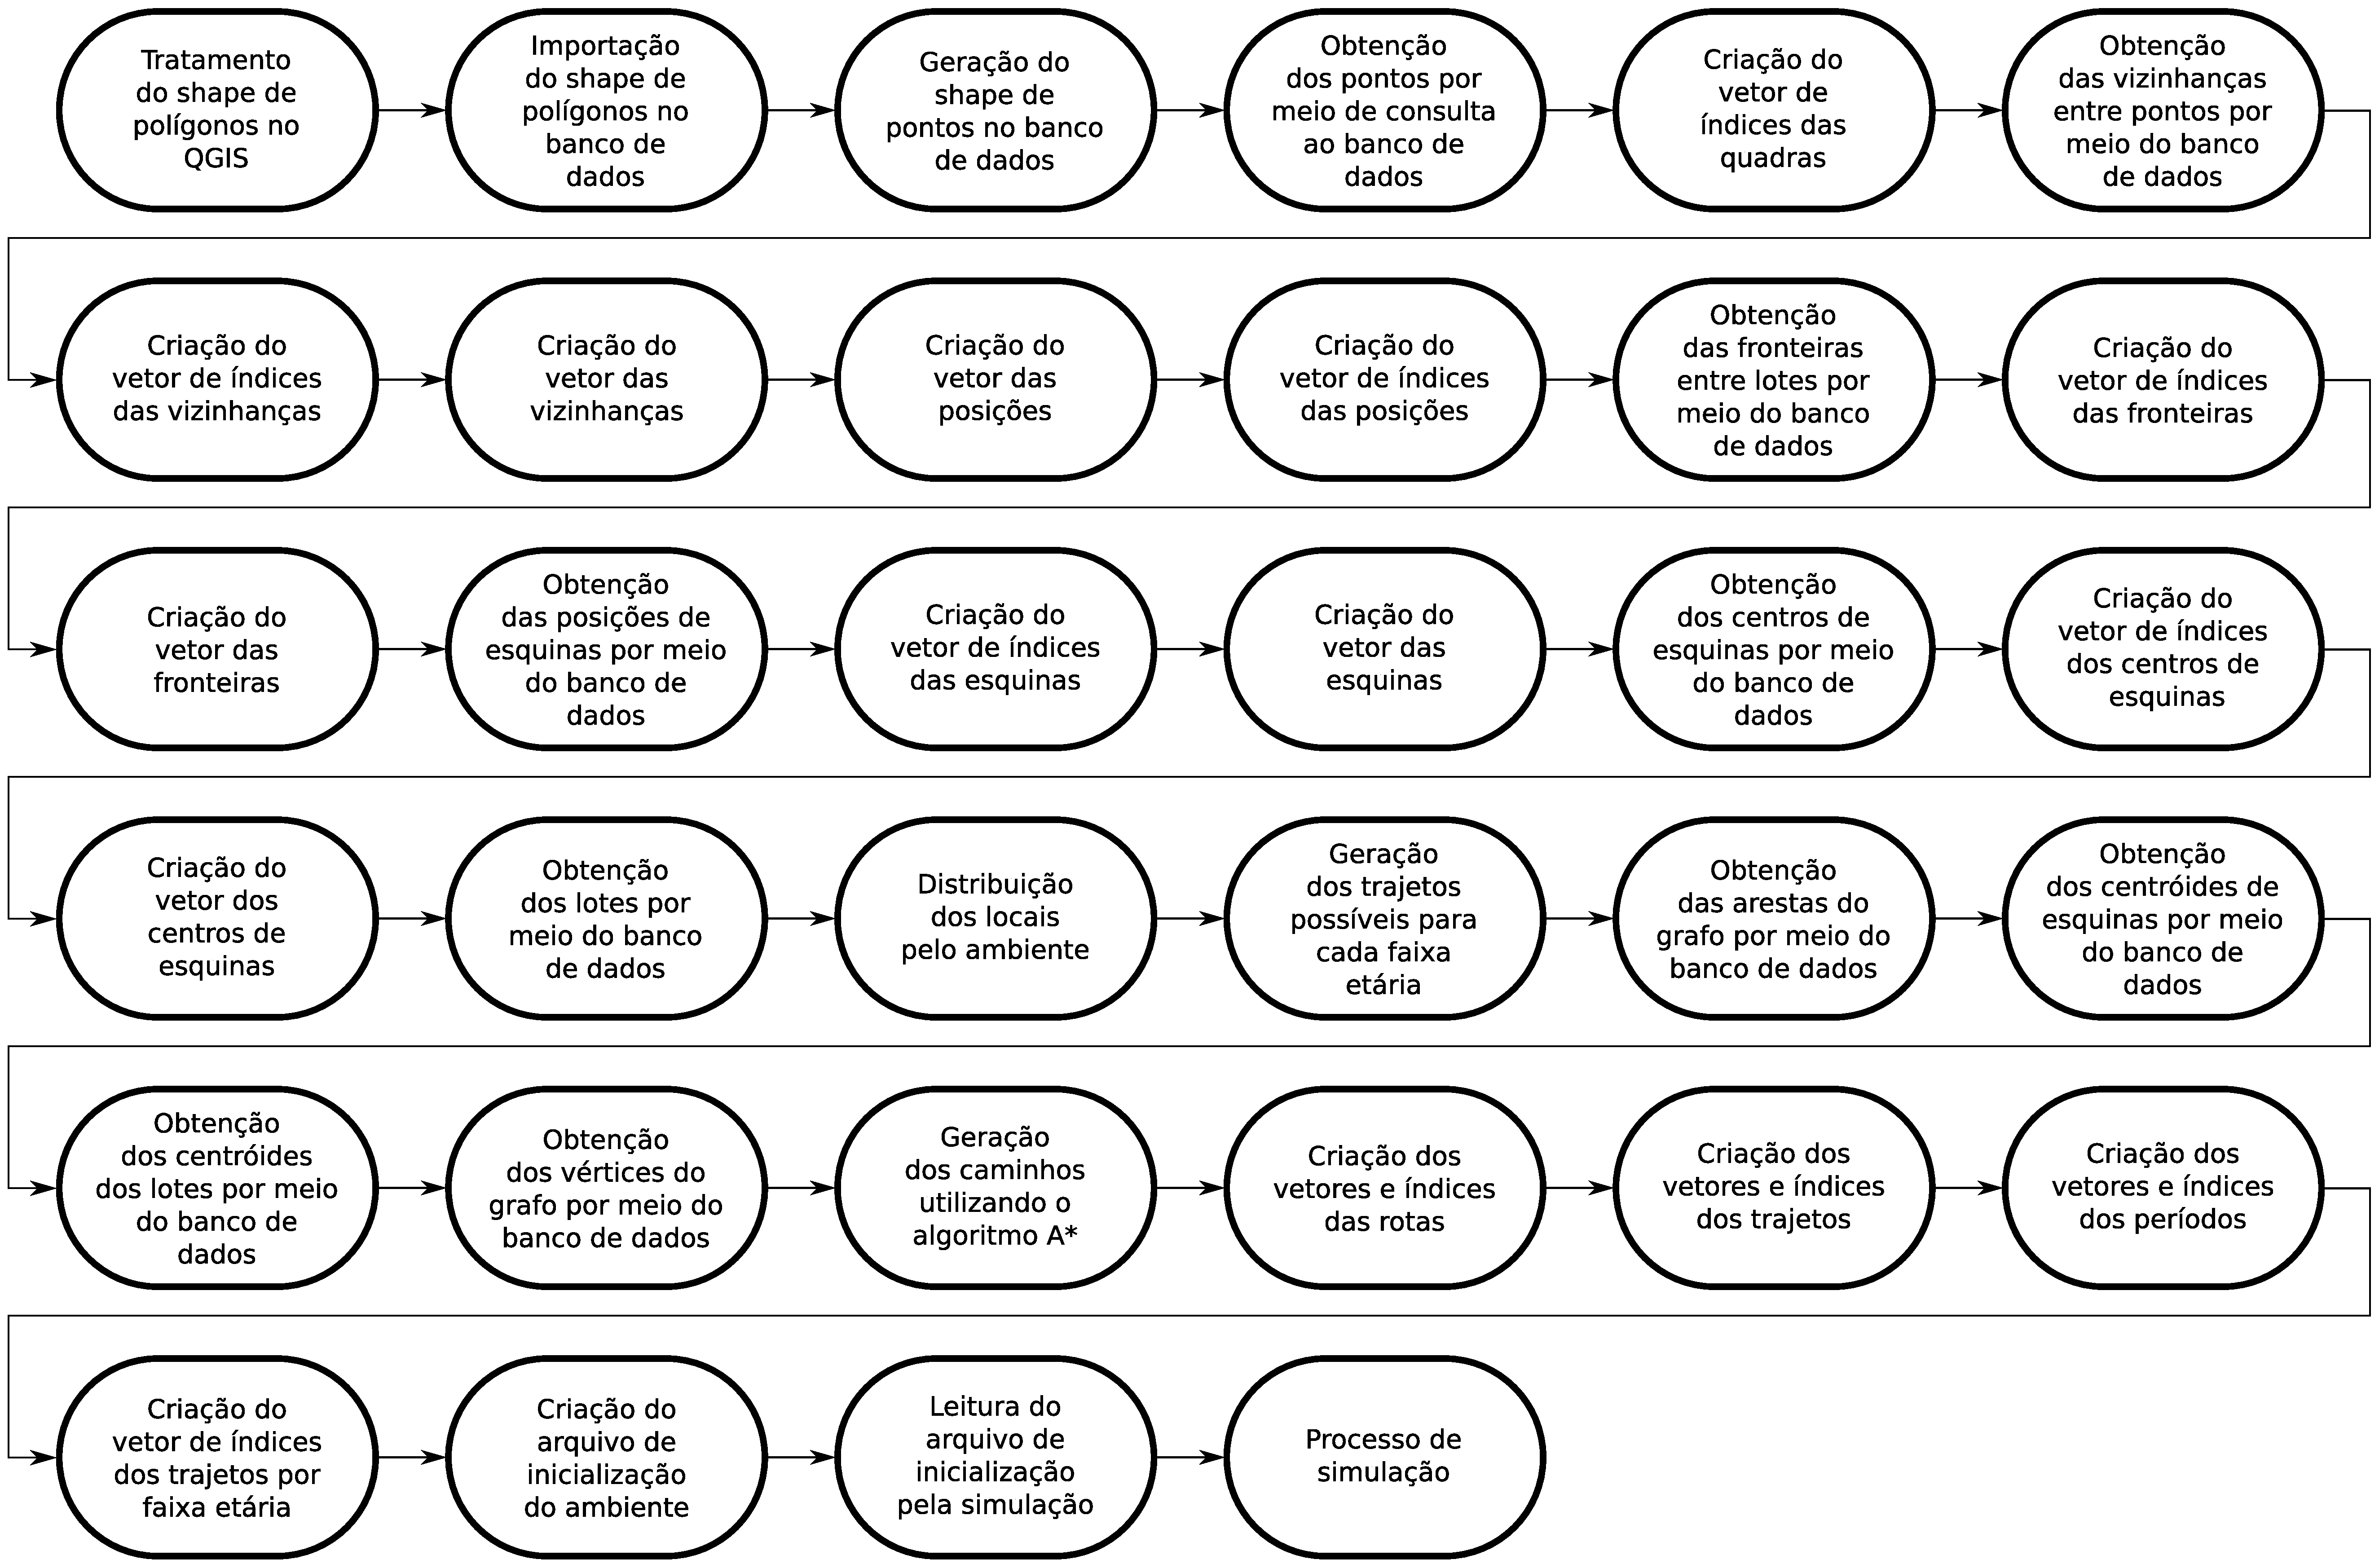
\includegraphics[width=0.7\textwidth]{Figuras/Simula/inicializacaoAmbiente.eps}
  \caption{Fluxograma das operações realizadas para a inicialização de um ambiente de simulação.}
  \label{fig:inicializacaoAmbiente}
\end{figure} 

\newpage

Abaixo são ilustrados os códigos fonte e algoritmos das rotinas responsáveis pela geração do arquivo de inicialização dos ambientes computacionais. Nos algoritmos os detalhes computacionais de implementação foram abstraídos para sintetizar de forma concisa os passos necessários à conclusão da rotina e transmitir de modo geral a ideia aplicada. No Código \ref{cod:mainAmb}, Algoritmo \ref{alg:mainAmb} e Figura \ref{fig:mainAmb} é apresentado o algoritmo principal que controla a geração do arquivo de inicialização de um ambiente. Este código é responsável pela execução da maioria das operações ilustradas na Figura \ref{fig:inicializacaoAmbiente}. 

\subsubsection{Função Principal}

\lstinputlisting[caption=Função Principal, label=cod:mainAmb, captionpos=b, language=Java]{Codigos/Simula/Fontes/main.java}

\begin{algorithm}[H]
   \SetAlgoLined   
   \input{Codigos/Simula/Algoritmos/main.txt}
   \caption{\textsc{Função Principal à Inicialização do Ambiente.}}
   \label{alg:mainAmb}
\end{algorithm}

\begin{figure}[H]
  \centering
  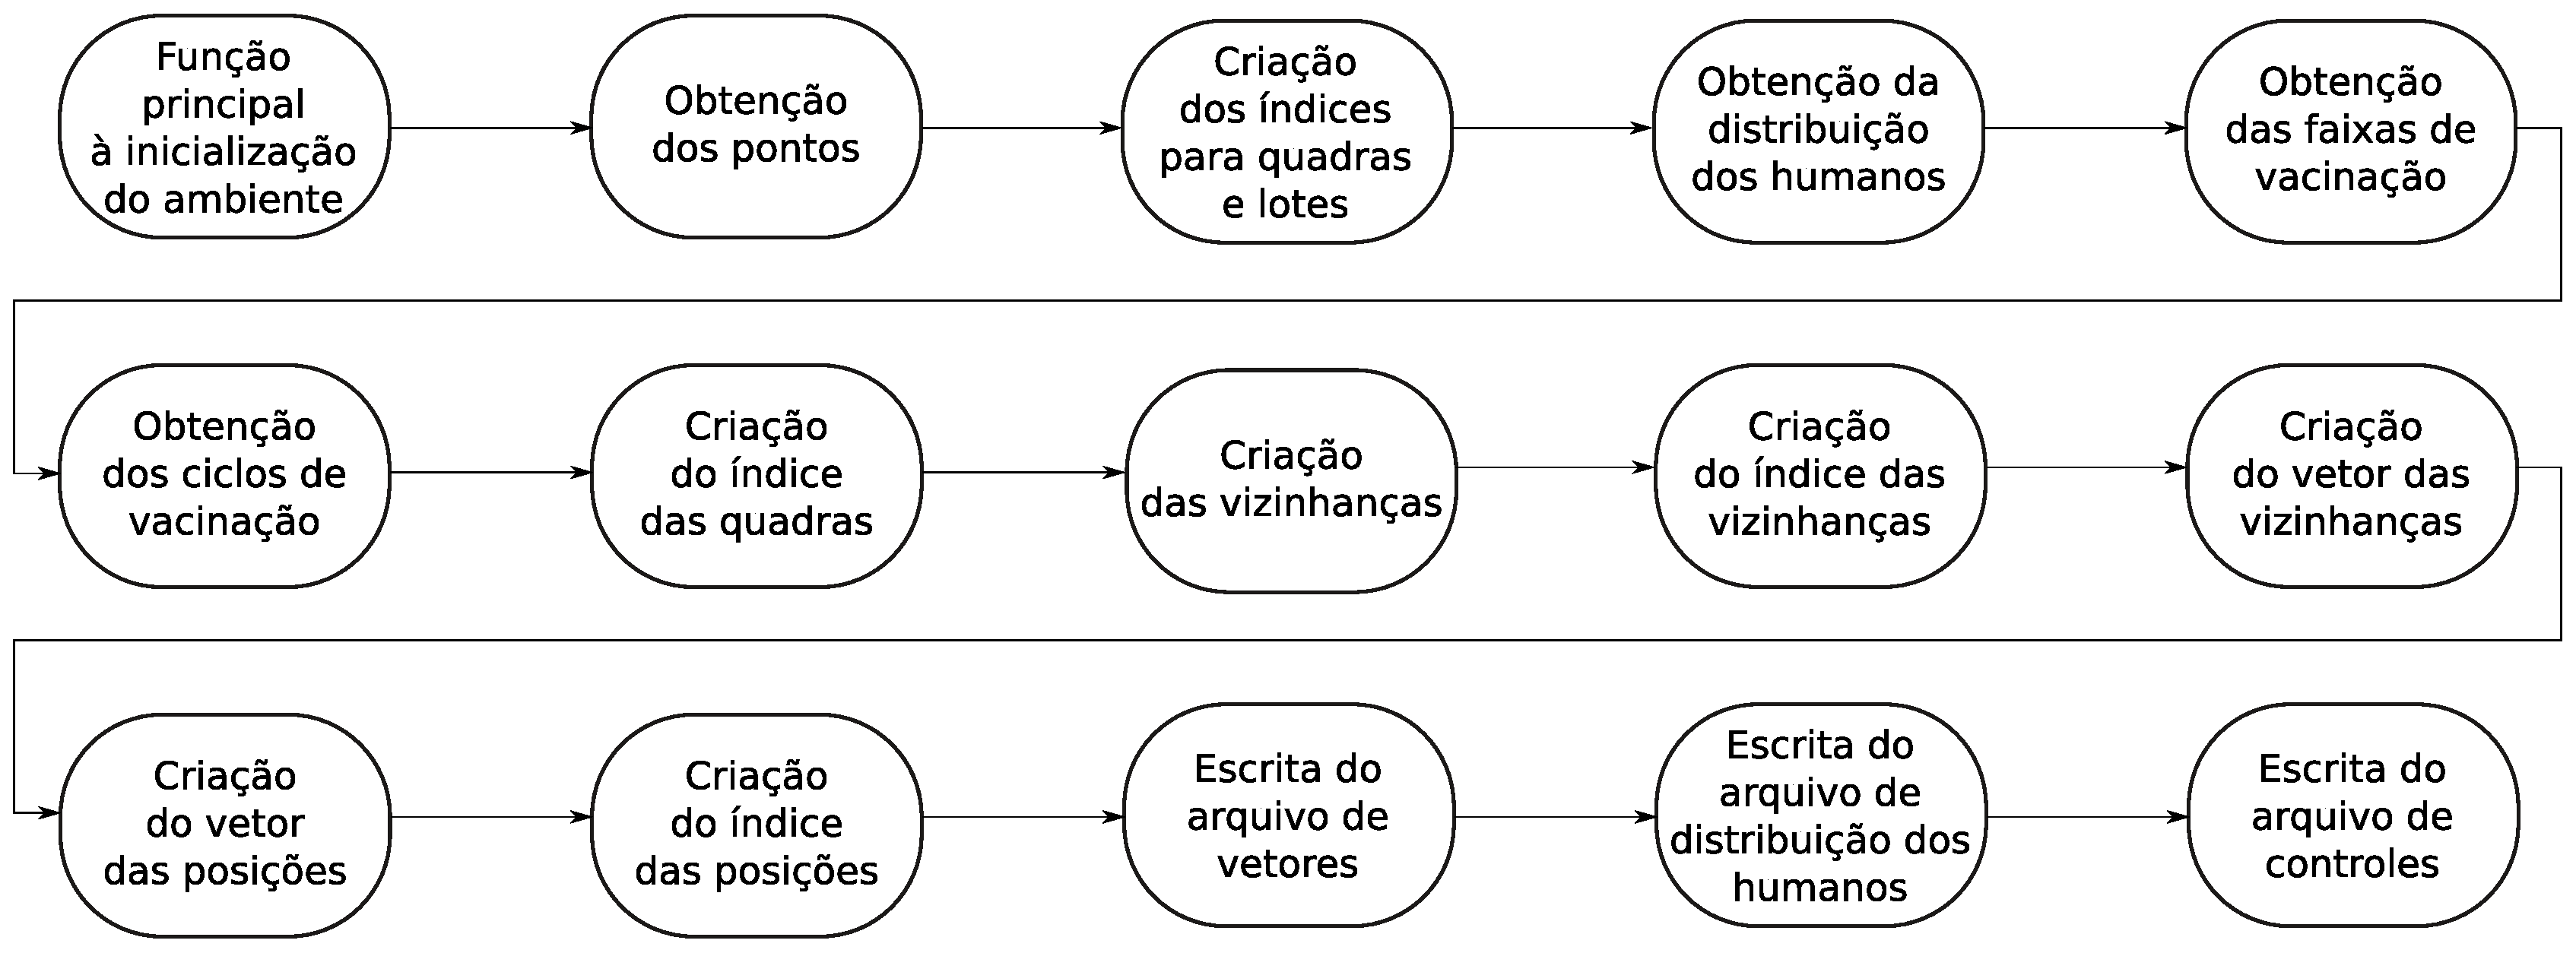
\includegraphics[width=1\textwidth]{Figuras/Simula/Fluxos/Main.eps}
  \caption{Função Principal à Inicialização do Ambiente.}
  \label{fig:mainAmb}
\end{figure} 

\newpage

\subsubsection{Função getConfig}

O Código \ref{cod:getConfig}, Algoritmo \ref{alg:getConfig} e Figura \ref{fig:getConfig} ilustram a rotina responsável pela obtenção dos parâmetros utilizados durante a geração de arquivos de entrada à simulação. Esta rotina realiza uma consulta ao banco de dados para obter as informações armazenadas na tabela denominada \textit{"config"}. Um exemplo é ilustrado na Tabela \ref{tab:config}. 

\lstinputlisting[caption=Função getConfig, label=cod:getConfig, captionpos=b, language=Java]{Codigos/Simula/Fontes/getConfig.java}

\begin{algorithm}[H]
   \SetAlgoLined   
   \input{Codigos/Simula/Algoritmos/getConfig.txt}
   \caption{\textsc{Função getConfig.}}
   \label{alg:getConfig}
\end{algorithm}

\begin{figure}[H]
  \centering
  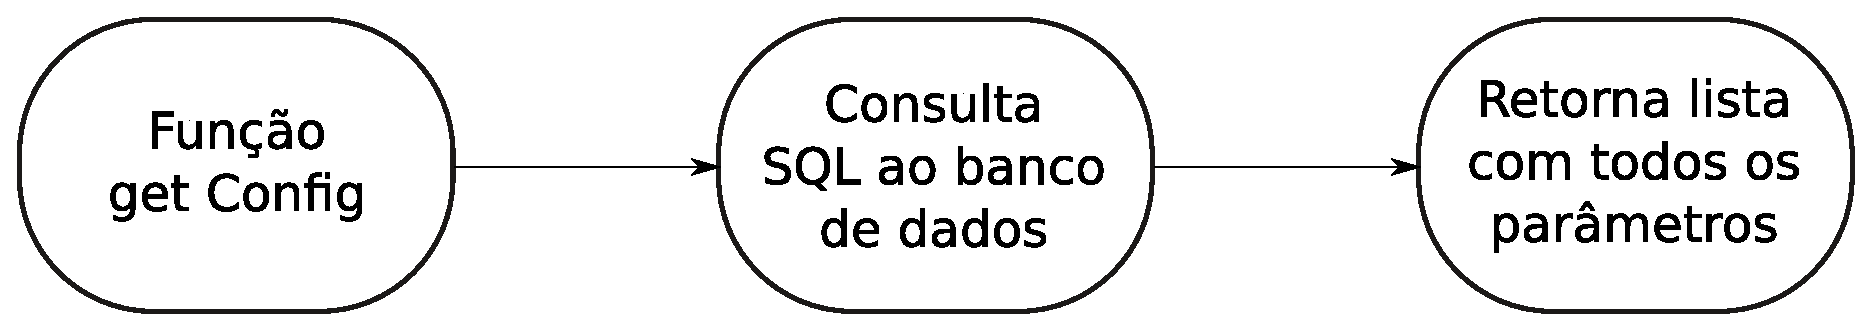
\includegraphics[width=0.7\textwidth]{Figuras/Simula/Fluxos/getConfig.eps}
  \caption{Função getConfig.}
  \label{fig:getConfig}
\end{figure} 

\newpage

\subsubsection{Função criarIndexQuadraseLotes}

O Código \ref{cod:criarIndexQuadraseLotes}, Algoritmo \ref{alg:criarIndexQuadraseLotes} e Figura \ref{fig:criarIndexQuadraseLotes}, ilustram a rotina responsável pela criação de estruturas auxiliares ao processo que geração do arquivo de inicialização do ambiente. Estas estruturas mapeiam as cadeias de caracteres dos identificadores de quadra e lotes em números inteiros, que são utilizados posteriormente pela simulação. Deste modo, durante a simulação as quadras e lotes são identificadas por números inteiros e não por seus identificadores originais. 

\lstinputlisting[caption=Função criarIndexQuadraseLotes, label=cod:criarIndexQuadraseLotes, captionpos=b, language=Java]{Codigos/Simula/Fontes/criarIndexQuadraseLotes.java}

\begin{algorithm}[H]
   \SetAlgoLined   
   \input{Codigos/Simula/Algoritmos/criarIndexQuadraseLotes.txt}
   \caption{\textsc{Função criarIndexQuadraseLotes.}}
   \label{alg:criarIndexQuadraseLotes}
\end{algorithm}

\begin{figure}[H]
  \centering
  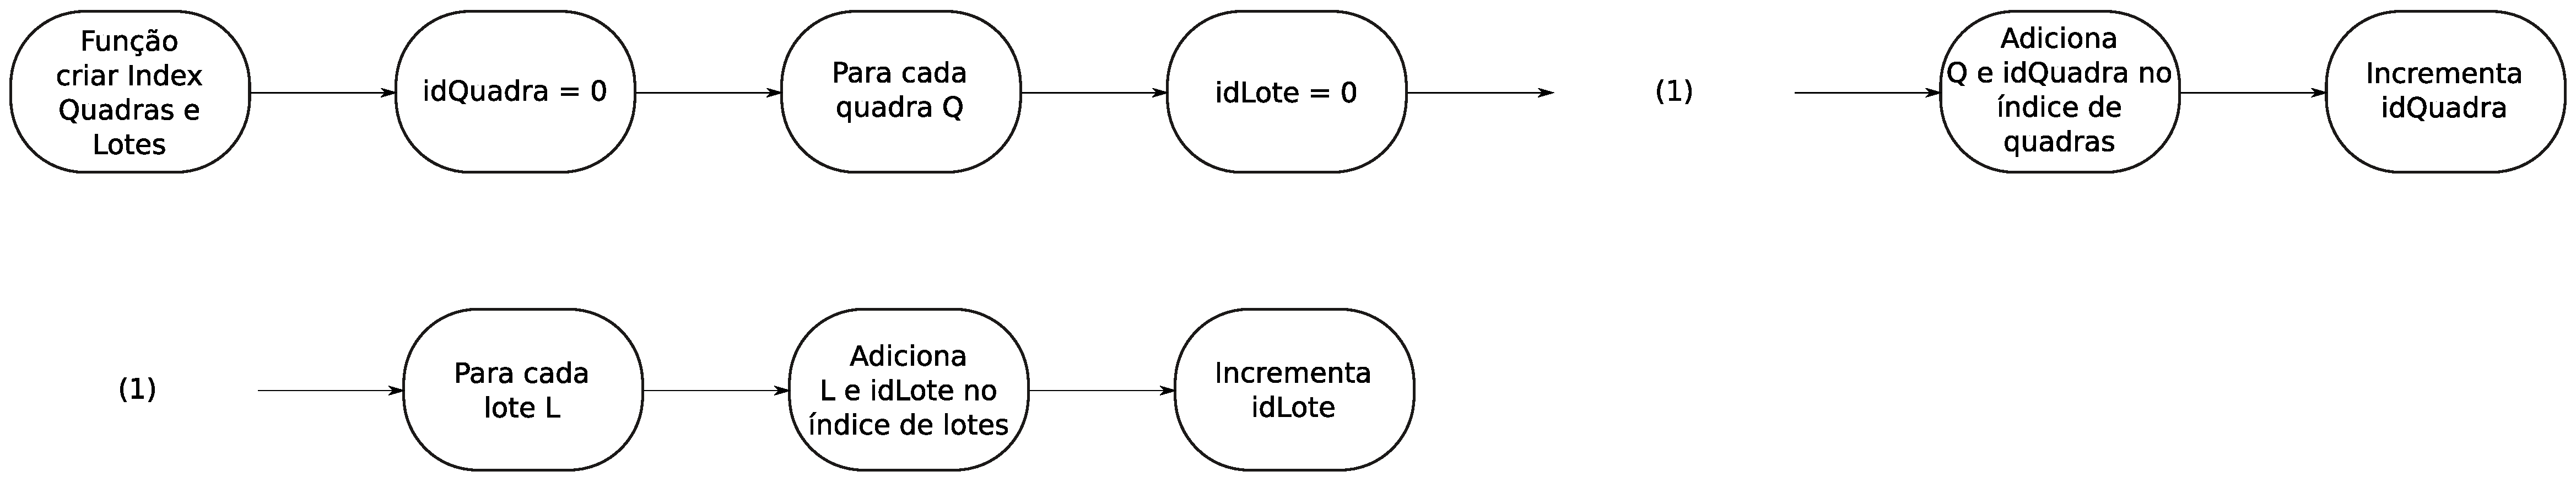
\includegraphics[width=1\textwidth]{Figuras/Simula/Fluxos/criarIndexQuadraseLotes.eps}
  \caption{Função criarIndexQuadraseLotes.}
  \label{fig:criarIndexQuadraseLotes}
\end{figure} 

\newpage

\subsubsection{Função gerarIndexQuadras}

O Código \ref{cod:gerarIndexQuadras}, Algoritmo \ref{alg:gerarIndexQuadras} e Figura \ref{fig:gerarIndexQuadras} ilustram a rotina responsável pela criação do vetor de índices para as quadras. Este índice é empregado à redução do tempo de execução das simulações por diminuir significativamente os espaços de busca em operações relacionadas ao ambiente computacional. Em posse do identificador numérico de uma quadra, esta estrutura de índice viabiliza o acesso aos lotes e vértices que pertencem à esta quadra em tempo constante. 

\lstinputlisting[caption=Função gerarIndexQuadras, label=cod:gerarIndexQuadras, captionpos=b, language=Java]{Codigos/Simula/Fontes/gerarIndexQuadras.java}

\begin{algorithm}[H]
   \SetAlgoLined   
   \input{Codigos/Simula/Algoritmos/gerarIndexQuadras.txt}
   \caption{\textsc{Função gerarIndexQuadras.}}
   \label{alg:gerarIndexQuadras}
\end{algorithm}

\begin{figure}[H]
  \centering
  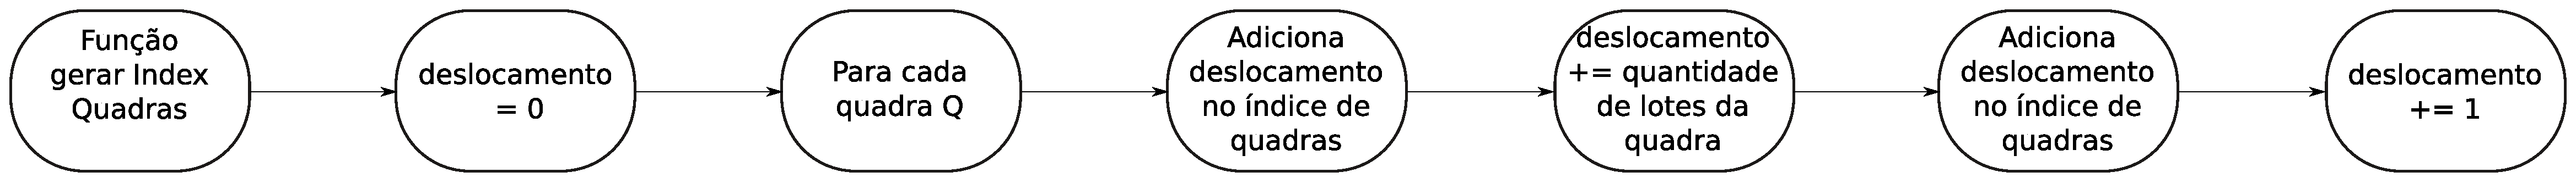
\includegraphics[width=1\textwidth]{Figuras/Simula/Fluxos/gerarIndexQuadras.eps}
  \caption{Função gerarIndexQuadras.}
  \label{fig:gerarIndexQuadras}
\end{figure} 

\newpage

\subsubsection{Função gerarVizinhancas}

O Código \ref{cod:gerarVizinhancas}, Algoritmo \ref{alg:gerarVizinhancas} e Figura \ref{fig:gerarVizinhancas} ilustram a rotina responsável pelo tratamento das vizinhanças de Moore entre os vértices obtidas pela rotina apresentada no Código \ref{cod:getVizinhancasMoorePontos} e Algoritmo \ref{alg:getVizinhancasMoorePontos}. É realizada uma operação de ordenação sobre o conjunto final de dados com o objetivo de organizar todas as vizinhanças em posições contíguas na estrutura. Deste modo, índices podem ser gerados e empregados à redução dos espaços de busca pela vizinhança de um vértice específico. 

\lstinputlisting[caption=Função gerarVizinhancas, label=cod:gerarVizinhancas, captionpos=b, language=Java]{Codigos/Simula/Fontes/gerarVizinhancas.java}

\begin{algorithm}[H]
   \SetAlgoLined   
   \input{Codigos/Simula/Algoritmos/gerarVizinhancas.txt}
   \caption{\textsc{Função gerarVizinhancas.}}
   \label{alg:gerarVizinhancas}
\end{algorithm}

\begin{figure}[H]
  \centering
  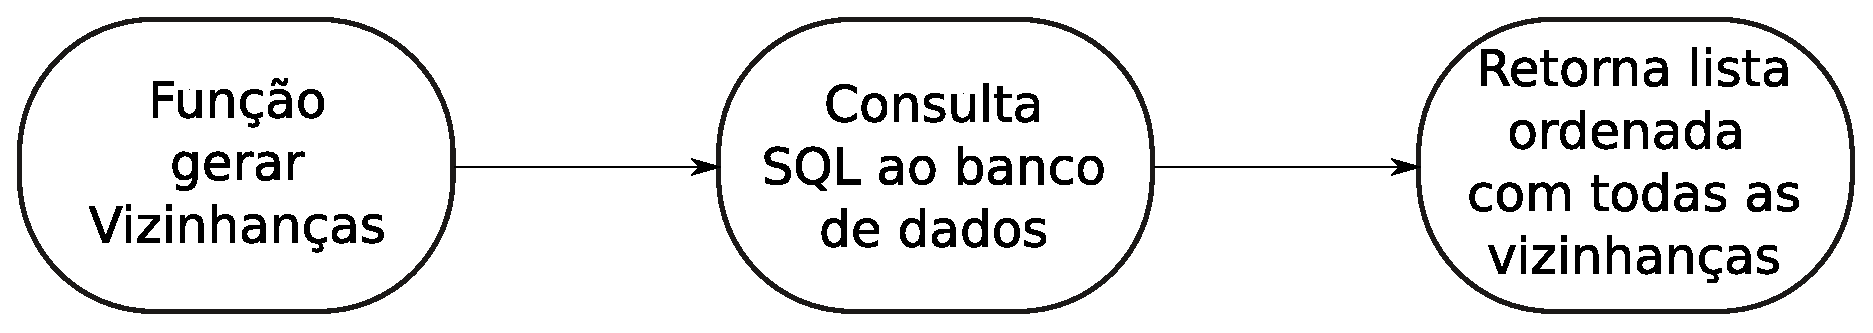
\includegraphics[width=0.7\textwidth]{Figuras/Simula/Fluxos/gerarVizinhancas.eps}
  \caption{Função gerarVizinhancas.}
  \label{fig:gerarVizinhancas}
\end{figure} 

\newpage

\subsubsection{Função getPontos}

O Código \ref{cod:getPontos}, Algoritmo \ref{alg:getPontos} e Figura \ref{fig:getPontos} ilustram a rotina responsável pela obtenção dos pontos do ambiente. Esta rotina realiza uma consulta ao banco de dados para obter as informações armazenadas na tabela com sufixo \textit{"\_pontos"}.   

\lstinputlisting[caption=Função getPontos, label=cod:getPontos, captionpos=b, language=Java]{Codigos/Simula/Fontes/getPontos.java}

\begin{algorithm}[H]
   \SetAlgoLined   
   \input{Codigos/Simula/Algoritmos/getPontos.txt}
   \caption{\textsc{Função getPontos.}}
   \label{alg:getPontos}
\end{algorithm}

\begin{figure}[H]
  \centering
  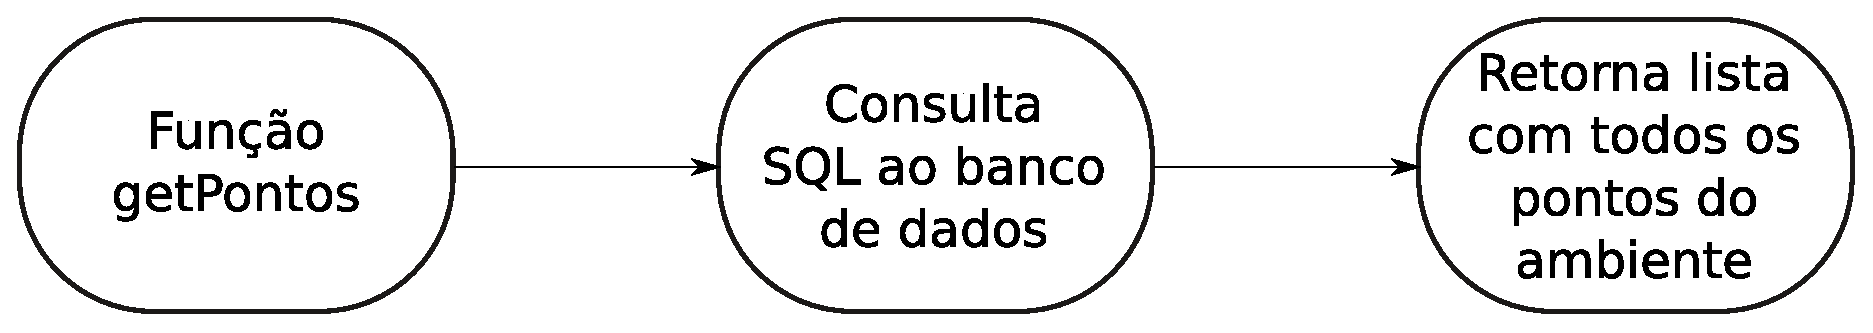
\includegraphics[width=0.7\textwidth]{Figuras/Simula/Fluxos/getPontos.eps}
  \caption{Função getPontos.}
  \label{fig:getPontos}
\end{figure} 

\newpage

\subsubsection{Função getFaixasEtariasVacinacao}

O Código \ref{cod:getFaixasEtariasVacinacao}, Algoritmo \ref{alg:getFaixasEtariasVacinacao} e Figura \ref{fig:getFaixasEtariasVacinacao} ilustram a rotina responsável pela obtenção das faixas etárias que serão utilizadas na rotina de vacinação dos agentes humanos. Esta rotina realiza uma consulta ao banco de dados para obter as informações armazenadas na tabela com sufixo \textit{"\_influenza\_faixasetariasvacinacao"}. Um exemplo é ilustrado na Tabela \ref{tab:cascavel_influenza_faixasetariasvacinacao}.

\lstinputlisting[caption=Função getFaixasEtariasVacinacao, label=cod:getFaixasEtariasVacinacao, captionpos=b, language=Java]{Codigos/Simula/Fontes/getFaixasEtariasVacinacao.java}

\begin{algorithm}[H]
   \SetAlgoLined   
   \input{Codigos/Simula/Algoritmos/getFaixasEtariasVacinacao.txt}
   \caption{\textsc{Função getFaixasEtariasVacinacao.}}
   \label{alg:getFaixasEtariasVacinacao}
\end{algorithm}

\begin{figure}[H]
  \centering
  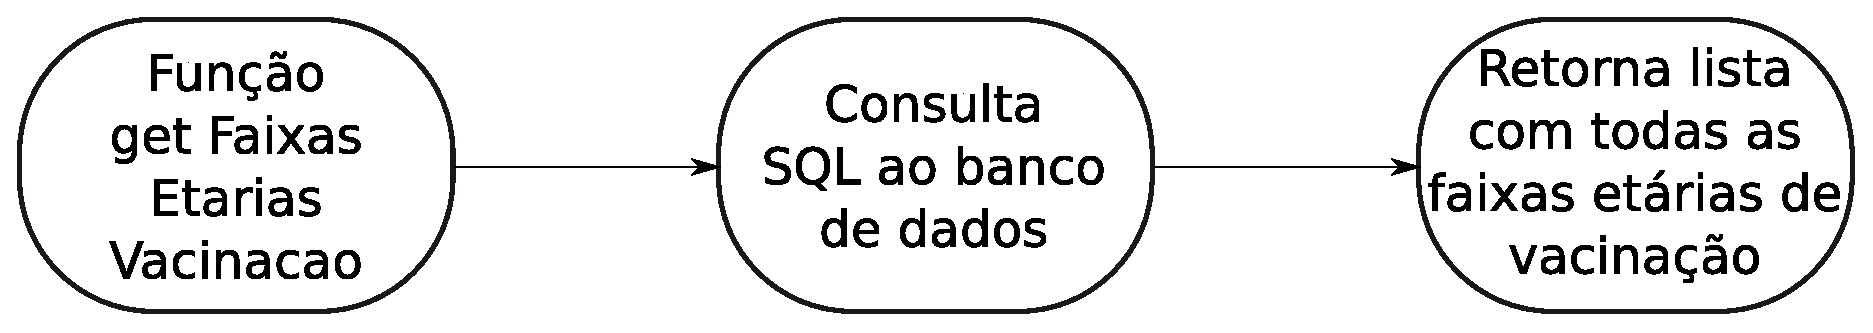
\includegraphics[width=0.7\textwidth]{Figuras/Simula/Fluxos/getFaixasEtariasVacinacao.eps}
  \caption{Função getFaixasEtariasVacinacao.}
  \label{fig:getFaixasEtariasVacinacao}
\end{figure} 

\newpage

\subsubsection{Função getCiclosVacinacao}

O Código \ref{cod:getCiclosVacinacao}, Algoritmo \ref{alg:getCiclosVacinacao} e Figura \ref{fig:getCiclosVacinacao} ilustram a rotina responsável pela obtenção dos ciclos de ocorrência das campanhas de vacinação dos agentes humanos. Esta rotina realiza uma consulta ao banco de dados para obter as informações armazenadas na tabela com sufixo \textit{"\_influenza\_ciclosvacinacao"}. Um exemplo é ilustrado na Tabela \ref{tab:cascavel_influenza_ciclosvacinacao}.

\lstinputlisting[caption=Função getCiclosVacinacao, label=cod:getCiclosVacinacao, captionpos=b, language=Java]{Codigos/Simula/Fontes/getCiclosVacinacao.java}

\begin{algorithm}[H]
   \SetAlgoLined   
   \input{Codigos/Simula/Algoritmos/getCiclosVacinacao.txt}
   \caption{\textsc{Função getCiclosVacinacao.}}
   \label{alg:getCiclosVacinacao}
\end{algorithm}

\begin{figure}[H]
  \centering
  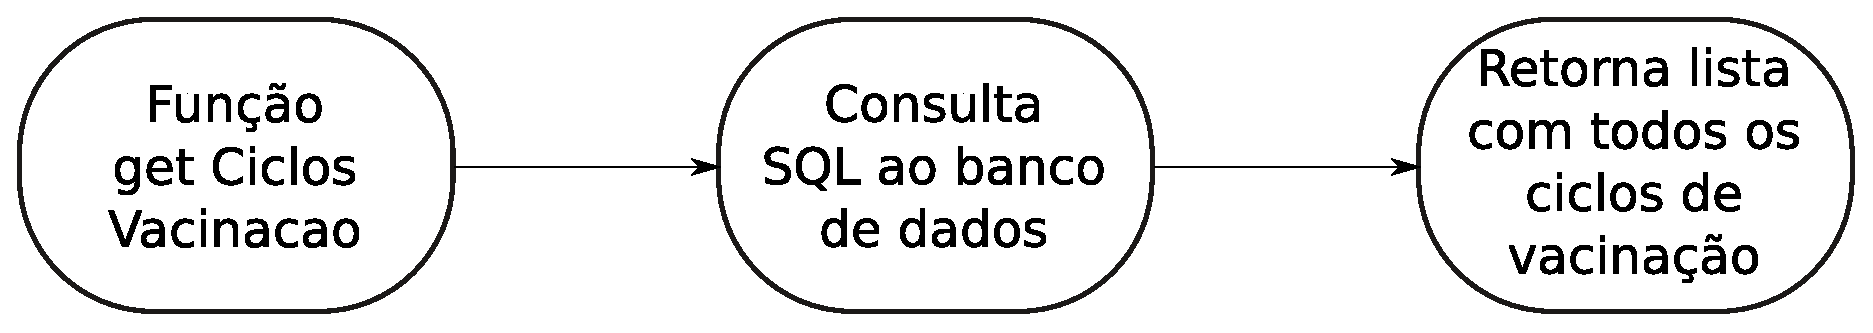
\includegraphics[width=0.7\textwidth]{Figuras/Simula/Fluxos/getCiclosVacinacao.eps}
  \caption{Função getCiclosVacinacao.}
  \label{fig:getCiclosVacinacao}
\end{figure} 

\newpage

\subsubsection{Função getDistribuicaoHumanos}

O Código \ref{cod:getDistribuicaoHumanos}, Algoritmo \ref{alg:getDistribuicaoHumanos} e Figura \ref{fig:getDistribuicaoHumanos} ilustram a rotina responsável pela obtenção da distribuição de agentes humanos durante a execução de simulações. Esta rotina realiza uma consulta ao banco de dados para obter as informações armazenadas na tabela com sufixo \textit{"\_influenza\_distribuicaohumanos"}. Um exemplo é ilustrado na Tabela \ref{tab:cascavel_influenza_distribuicaohumanos}.

\lstinputlisting[caption=Função getDistribuicaoHumanos, label=cod:getDistribuicaoHumanos, captionpos=b, language=Java]{Codigos/Simula/Fontes/getDistribuicaoHumanos.java}

\begin{algorithm}[H]
   \SetAlgoLined   
   \input{Codigos/Simula/Algoritmos/getDistribuicaoHumanos.txt}
   \caption{\textsc{Função getDistribuicaoHumanos.}}
   \label{alg:getDistribuicaoHumanos}
\end{algorithm}

\begin{figure}[H]
  \centering
  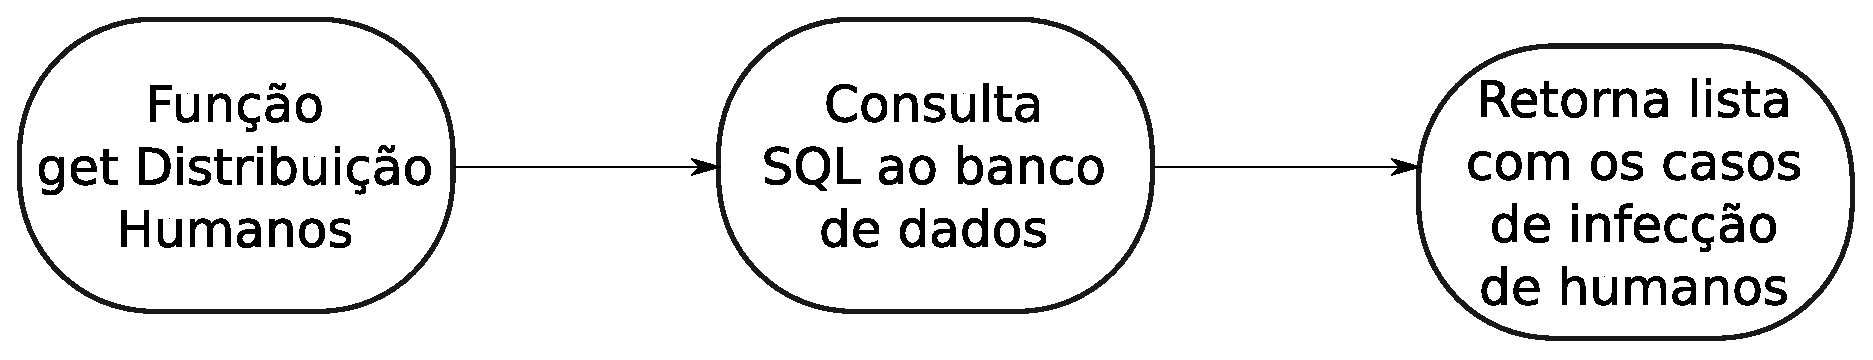
\includegraphics[width=0.7\textwidth]{Figuras/Simula/Fluxos/getDistribuicaoHumanos.eps}
  \caption{Função getDistribuicaoHumanos.}
  \label{fig:getDistribuicaoHumanos}
\end{figure} 

\newpage

\subsubsection{Função getVizinhancasMoorePontos}

O Código \ref{cod:getVizinhancasMoorePontos}, Algoritmo \ref{alg:getVizinhancasMoorePontos} e Figura \ref{fig:getVizinhancasMoorePontos} ilustram a rotina responsável pela obtenção das vizinhanças de Moore entre os vértices. Esta rotina realiza uma consulta ao banco de dados para obter as informações armazenadas na tabela com sufixo \textit{"\_vizinhancasmoorepontos"}. A função de criação e um exemplo da tabela são ilustrados no Código \ref{cod:sql_getVizinhancasMoorePontos} e Tabela \ref{tab:cascavel_vizinhancasmoorepontos}.  

\lstinputlisting[caption=Função getVizinhancasMoorePontos, label=cod:getVizinhancasMoorePontos, captionpos=b, language=Java]{Codigos/Simula/Fontes/getVizinhancasMoorePontos.java}

\begin{algorithm}[H]
   \SetAlgoLined   
   \input{Codigos/Simula/Algoritmos/getVizinhancasMoorePontos.txt}
   \caption{\textsc{Função getVizinhancasMoorePontos.}}
   \label{alg:getVizinhancasMoorePontos}
\end{algorithm}

\begin{figure}[H]
  \centering
  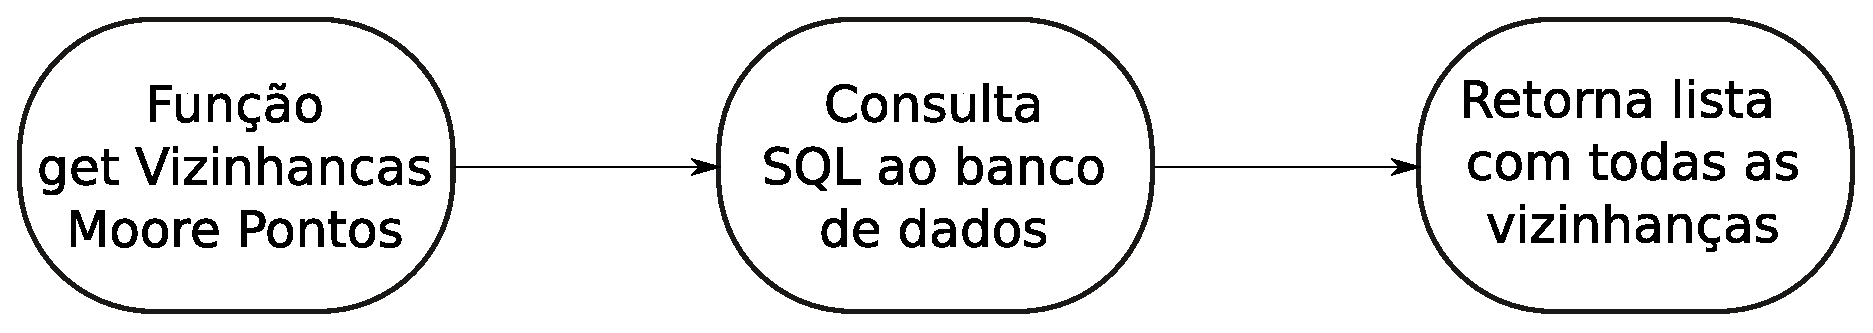
\includegraphics[width=0.7\textwidth]{Figuras/Simula/Fluxos/getVizinhancasMoorePontos.eps}
  \caption{Função getVizinhancasMoorePontos.}
  \label{fig:getVizinhancasMoorePontos}
\end{figure} 

\newpage

\subsubsection{Função gerarIndexVizinhancas}

O Código \ref{cod:gerarIndexVizinhancas}, Algoritmo \ref{alg:gerarIndexVizinhancas} e Figura \ref{fig:gerarIndexVizinhancas} ilustram a rotina responsável pela geração dos índices para as estruturas de vizinhanças entre vértices. Este índice é gerado à nível de lote e utilizado juntamente com o índice de quadras, viabilizando a recuperação rápida das vizinhanças de Moore entre vértices se conhecidos os identificadores numéricos da quadra e do lote. 

\lstinputlisting[caption=Função gerarIndexVizinhancas, label=cod:gerarIndexVizinhancas, captionpos=b, language=Java]{Codigos/Simula/Fontes/gerarIndexVizinhancas.java}

\begin{algorithm}[H]
   \SetAlgoLined   
   \input{Codigos/Simula/Algoritmos/gerarIndexVizinhancas.txt}
   \caption{\textsc{Função gerarIndexVizinhancas.}}
   \label{alg:gerarIndexVizinhancas}
\end{algorithm}

\begin{figure}[H]
  \centering
  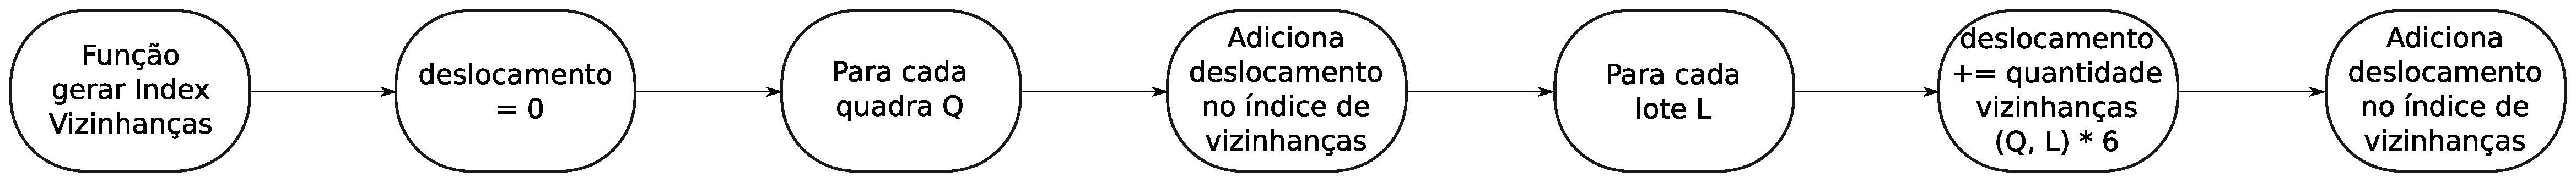
\includegraphics[width=1\textwidth]{Figuras/Simula/Fluxos/gerarIndexVizinhancas.eps}
  \caption{Função gerarIndexVizinhancas.}
  \label{fig:gerarIndexVizinhancas}
\end{figure} 

\newpage

\subsubsection{Função gerarVetorVizinhancas}

O Código \ref{cod:gerarVetorVizinhancas}, Algoritmo \ref{alg:gerarVetorVizinhancas} e Figura \ref{fig:gerarVetorVizinhancas} ilustram a rotina responsável pela geração do vetor que armazena todas as vizinhanças entre vértices. Nesta rotina as informações pertencentes às vizinhanças, armazenadas em classes, são dispostas e organizadas em uma estrutura linear, que é mapeada posteriormente à um vetor de tipo homogêneo, facilitando à cópia de dados à GPU.

\lstinputlisting[caption=Função gerarVetorVizinhancas, label=cod:gerarVetorVizinhancas, captionpos=b, language=Java]{Codigos/Simula/Fontes/gerarVetorVizinhancas.java}

\begin{algorithm}[H]
   \SetAlgoLined   
   \input{Codigos/Simula/Algoritmos/gerarVetorVizinhancas.txt}
   \caption{\textsc{Função gerarVetorVizinhancas.}}
   \label{alg:gerarVetorVizinhancas}
\end{algorithm}

\begin{figure}[H]
  \centering
  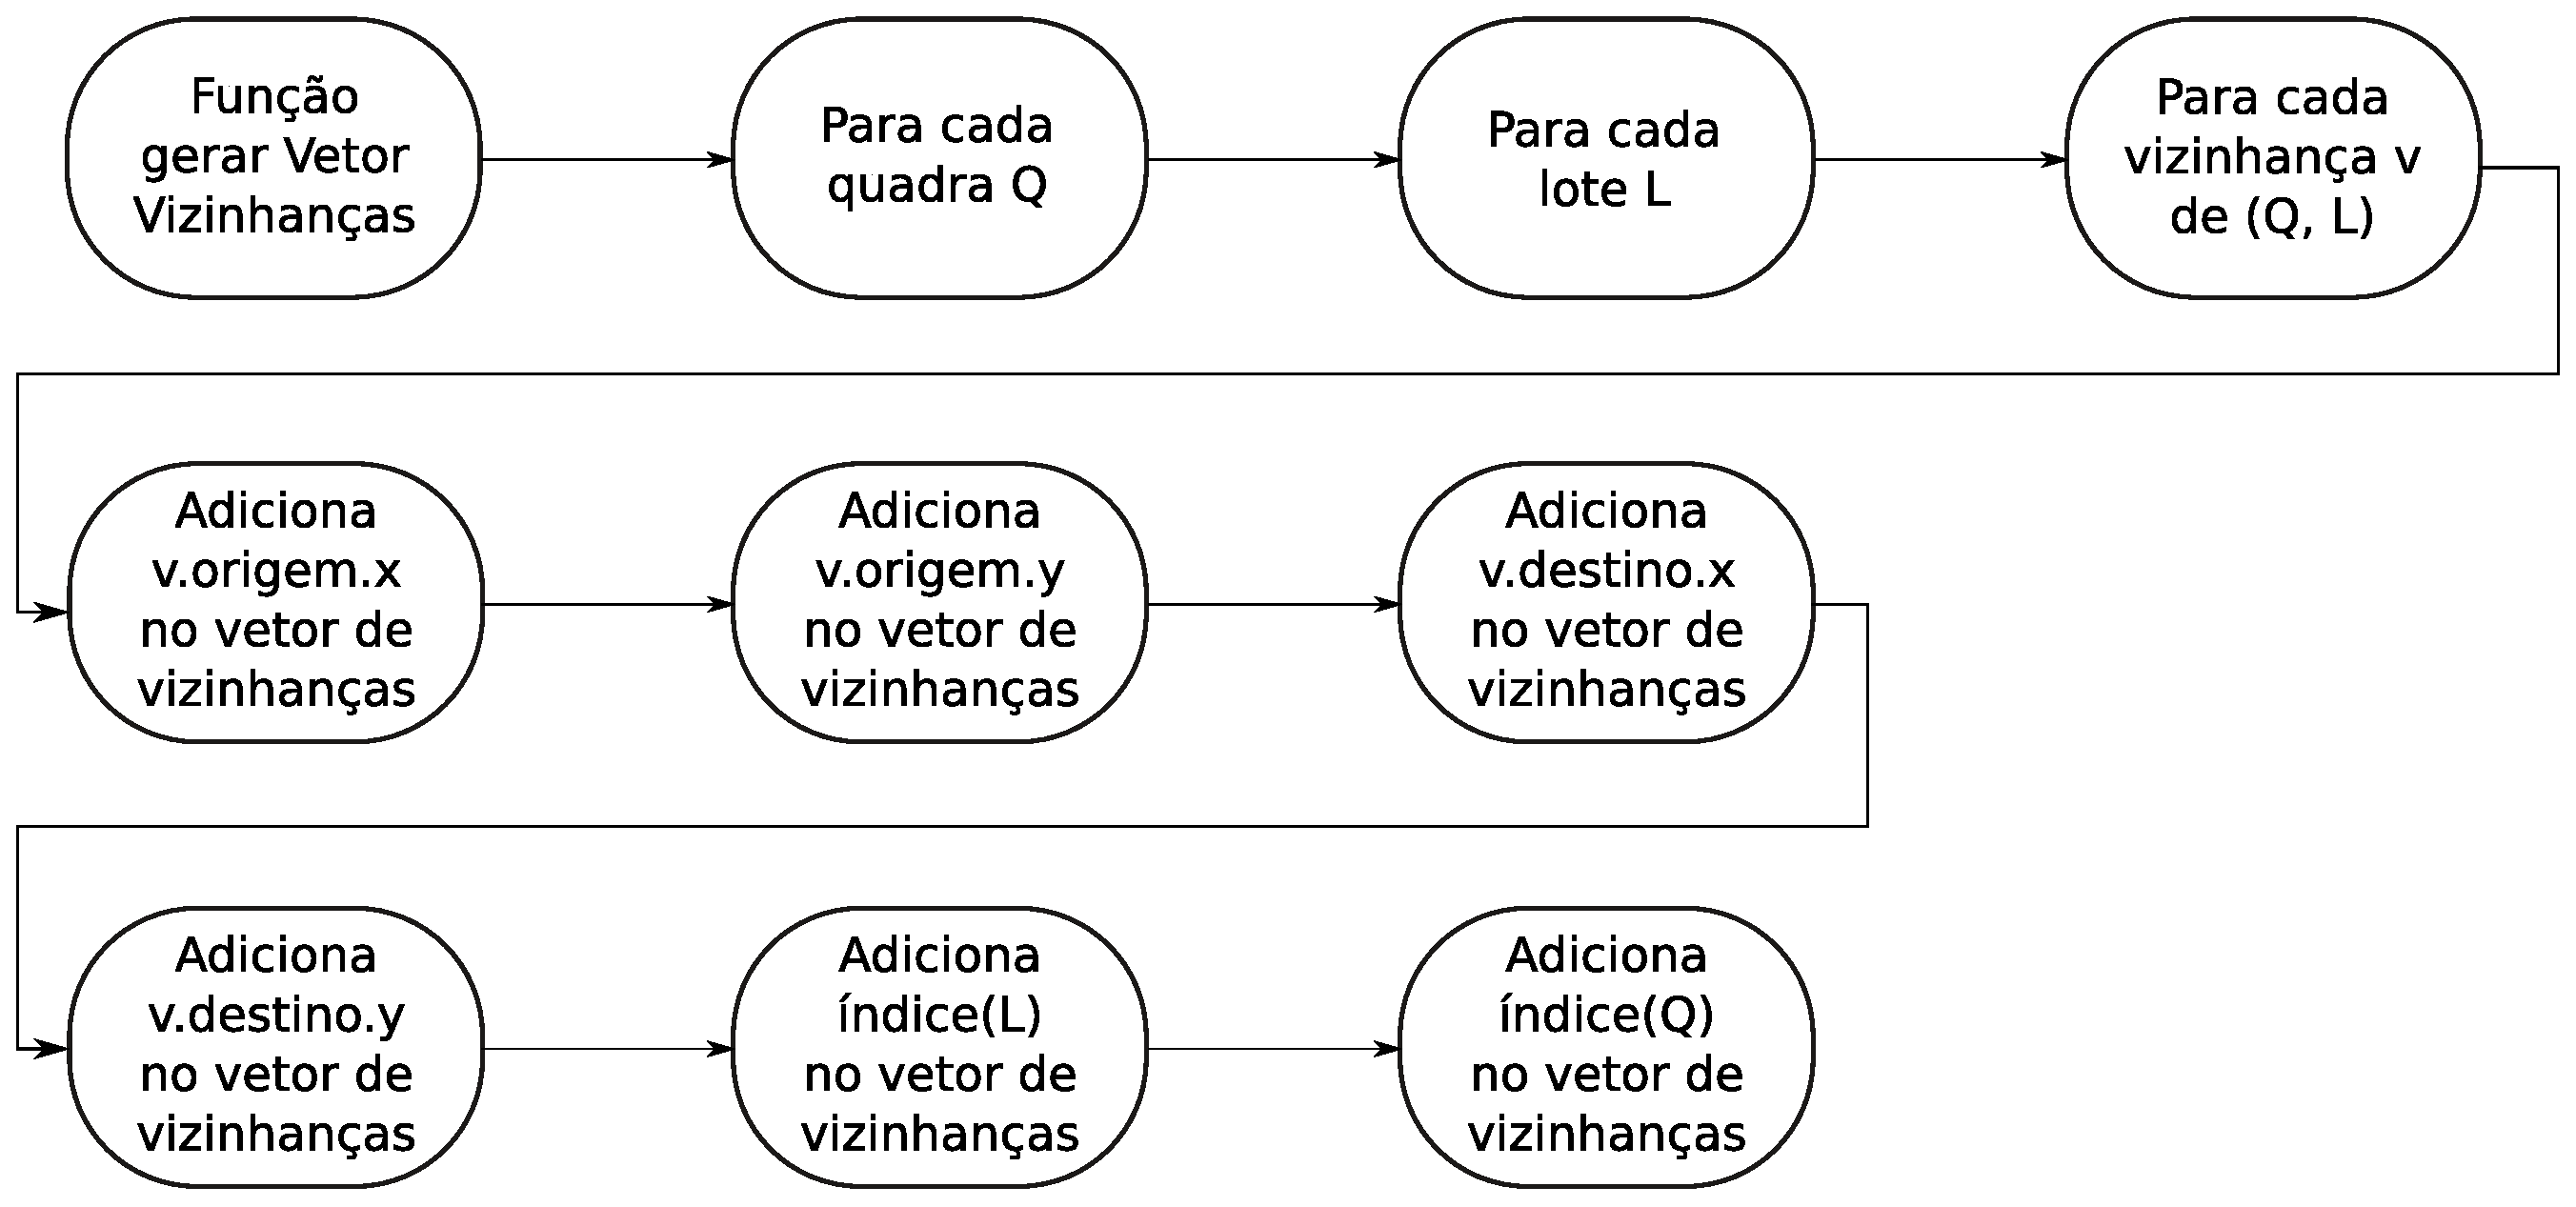
\includegraphics[width=0.8\textwidth]{Figuras/Simula/Fluxos/gerarVetorVizinhancas.eps}
  \caption{Função gerarVetorVizinhancas.}
  \label{fig:gerarVetorVizinhancas}
\end{figure} 

\newpage

\subsubsection{Função gerarVetorPosicoes}

O Código \ref{cod:gerarVetorPosicoes}, Algoritmo \ref{alg:gerarVetorPosicoes} e Figura \ref{fig:gerarVetorPosicoes} ilustram a rotina responsável pela geração do vetor que armazena todos os vértices. Nesta rotina os vértices armazenados em classes são dispostos e organizados em uma estrutura linear, que é mapeada posteriormente à um vetor de tipo homogêneo, facilitando à cópia de dados à GPU.

\lstinputlisting[caption=Função gerarVetorPosicoes, label=cod:gerarVetorPosicoes, captionpos=b, language=Java]{Codigos/Simula/Fontes/gerarVetorPosicoes.java}

\begin{algorithm}[H]
   \SetAlgoLined   
   \input{Codigos/Simula/Algoritmos/gerarVetorPosicoes.txt}
   \caption{\textsc{Função gerarVetorPosicoes.}}
   \label{alg:gerarVetorPosicoes}
\end{algorithm}

\begin{figure}[H]
  \centering
  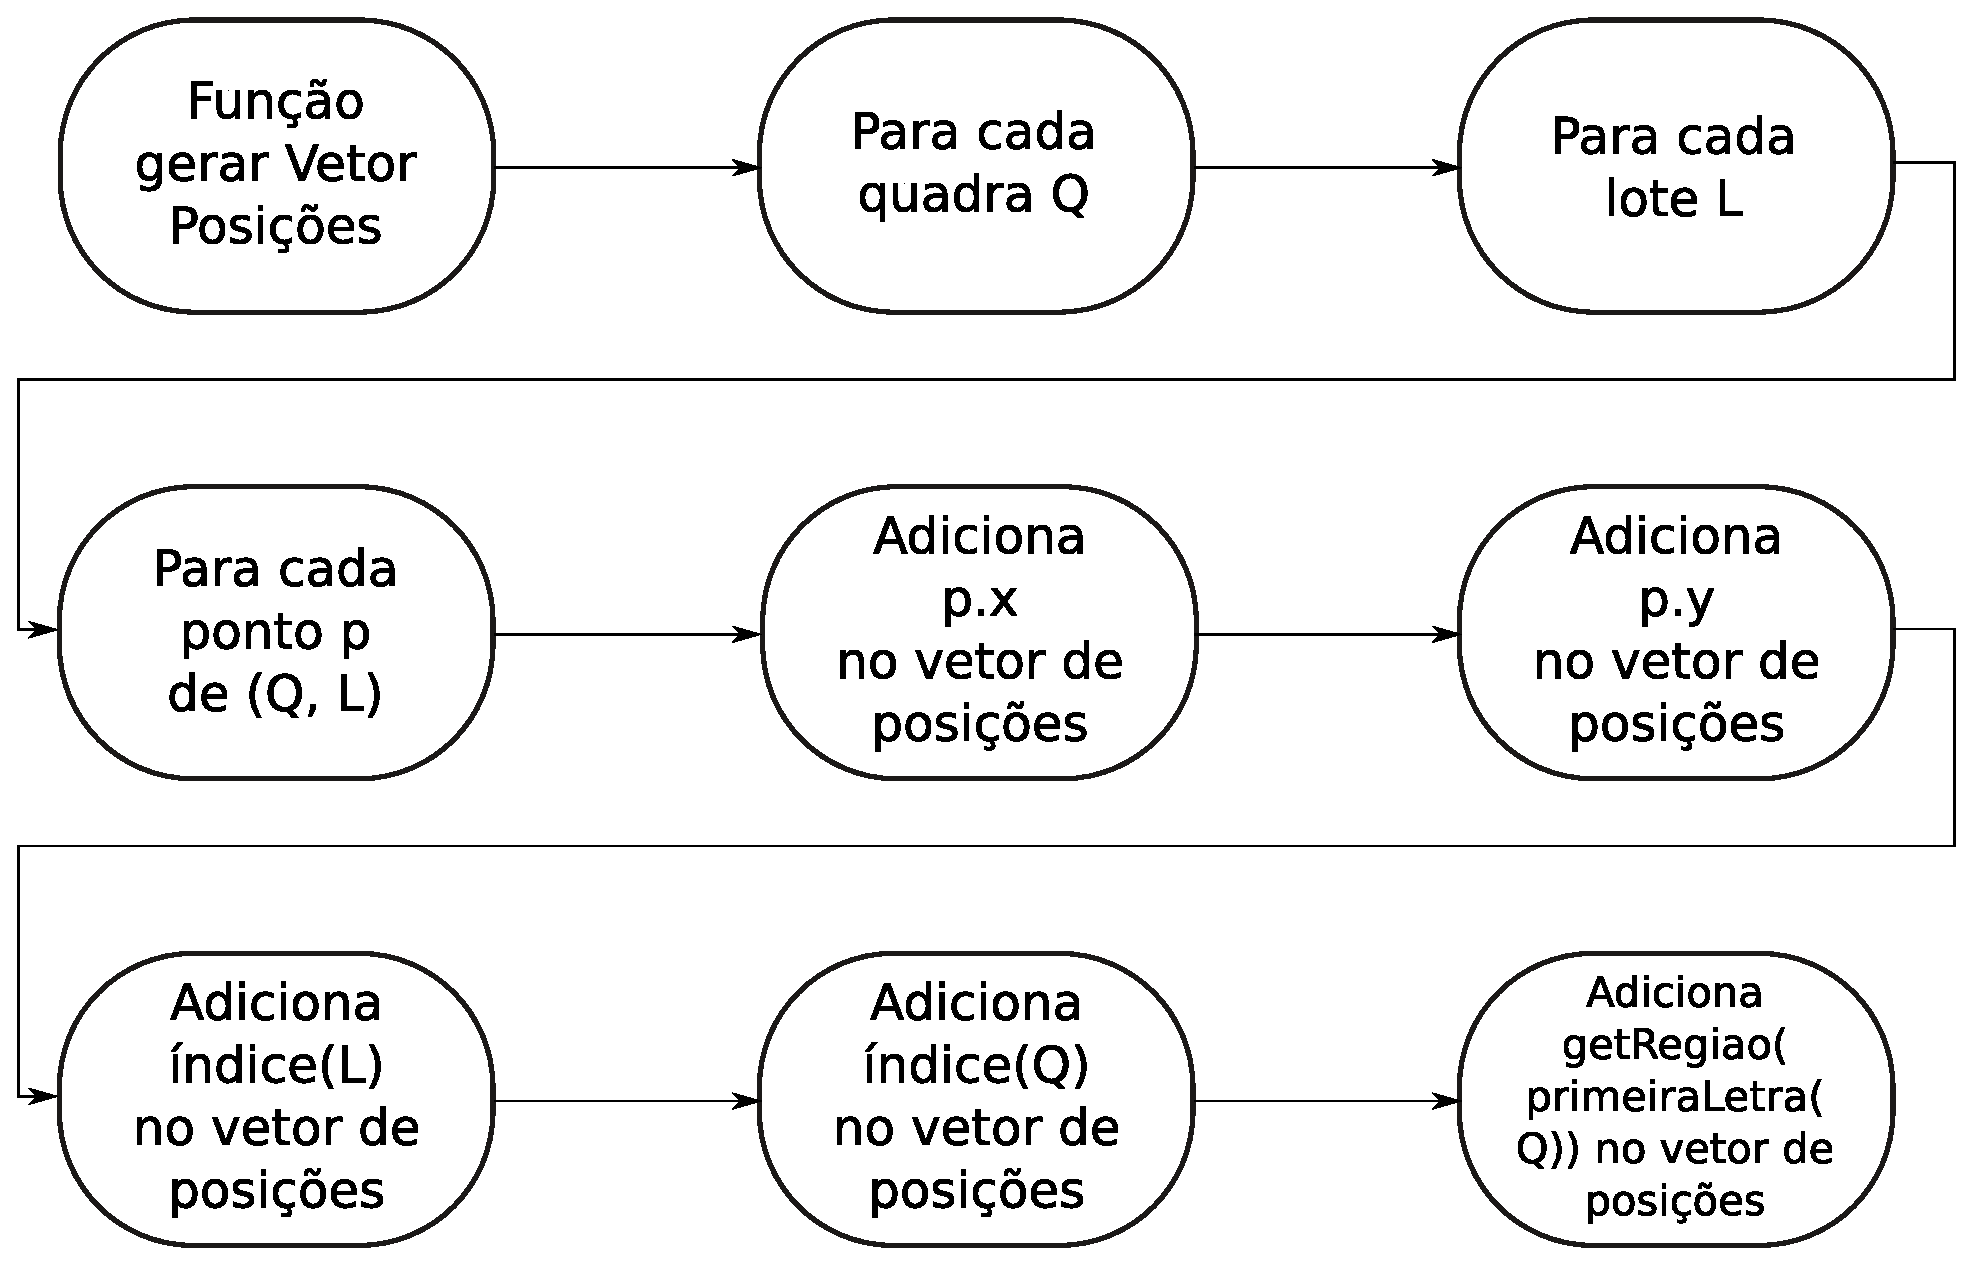
\includegraphics[width=0.8\textwidth]{Figuras/Simula/Fluxos/gerarVetorPosicoes.eps}
  \caption{Função gerarVetorPosicoes.}
  \label{fig:gerarVetorPosicoes}
\end{figure} 

\newpage

\subsubsection{Função gerarIndexPosicoes}

O Código \ref{cod:gerarIndexPosicoes}, Algoritmo \ref{alg:gerarIndexPosicoes} e Figura \ref{fig:gerarIndexPosicoes} ilustram a rotina responsável pela geração dos índices aos vértices do ambiente. Este índice é gerado à nível de lote e utilizado juntamente com o índice de quadras, viabilizando a recuperação rápida de todos vértices pertencentes à um lote de uma quadra. Os identificadores numéricos da quadra e do lote são utilizados como índices. 

\lstinputlisting[caption=Função gerarIndexPosicoes, label=cod:gerarIndexPosicoes, captionpos=b, language=Java]{Codigos/Simula/Fontes/gerarIndexPosicoes.java}

\begin{algorithm}[H]
   \SetAlgoLined   
   \input{Codigos/Simula/Algoritmos/gerarIndexPosicoes.txt}
   \caption{\textsc{Função gerarIndexPosicoes.}}
   \label{alg:gerarIndexPosicoes}
\end{algorithm}

\begin{figure}[H]
  \centering
  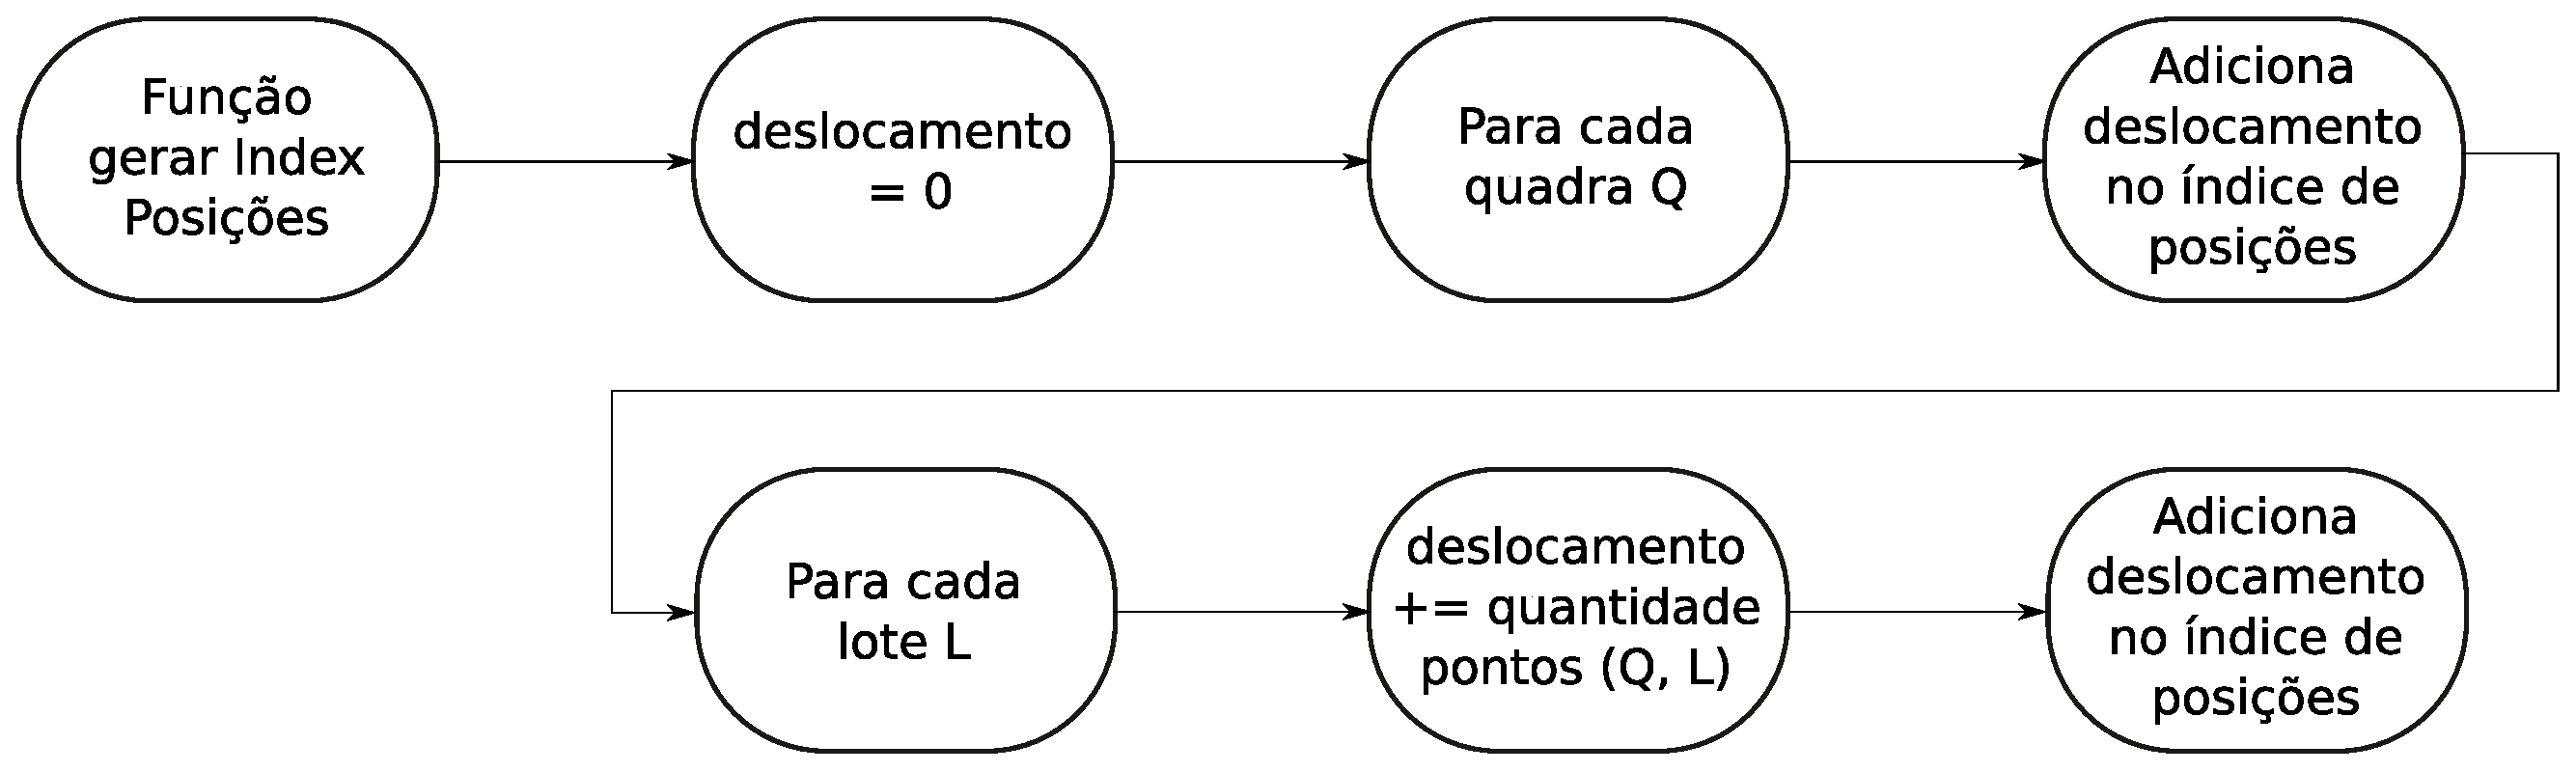
\includegraphics[width=0.8\textwidth]{Figuras/Simula/Fluxos/gerarIndexPosicoes.eps}
  \caption{Função gerarIndexPosicoes.}
  \label{fig:gerarIndexPosicoes}
\end{figure} 

\newpage

\subsubsection{Função salvarArquivoVetores}

O Código \ref{cod:salvarArquivoVetores}, Algoritmo \ref{alg:salvarArquivoVetores} e Figura \ref{fig:salvarArquivoVetores} ilustram a rotina responsável pela escrita do arquivo contendo todas as informações relacionadas ao ambiente. As informações ambientais são escritas no arquivo denominado \textit{"Vetores.csv"}.

\lstinputlisting[caption=Função salvarArquivoVetores, label=cod:salvarArquivoVetores, captionpos=b, language=Java]{Codigos/Simula/Fontes/salvarArquivoVetores.java}

\newpage

\begin{algorithm}[H]
   \SetAlgoLined   
   \input{Codigos/Simula/Algoritmos/salvarArquivoVetores.txt}
   \caption{\textsc{Função salvarArquivoVetores.}}
   \label{alg:salvarArquivoVetores}
\end{algorithm}

\begin{figure}[H]
  \centering
  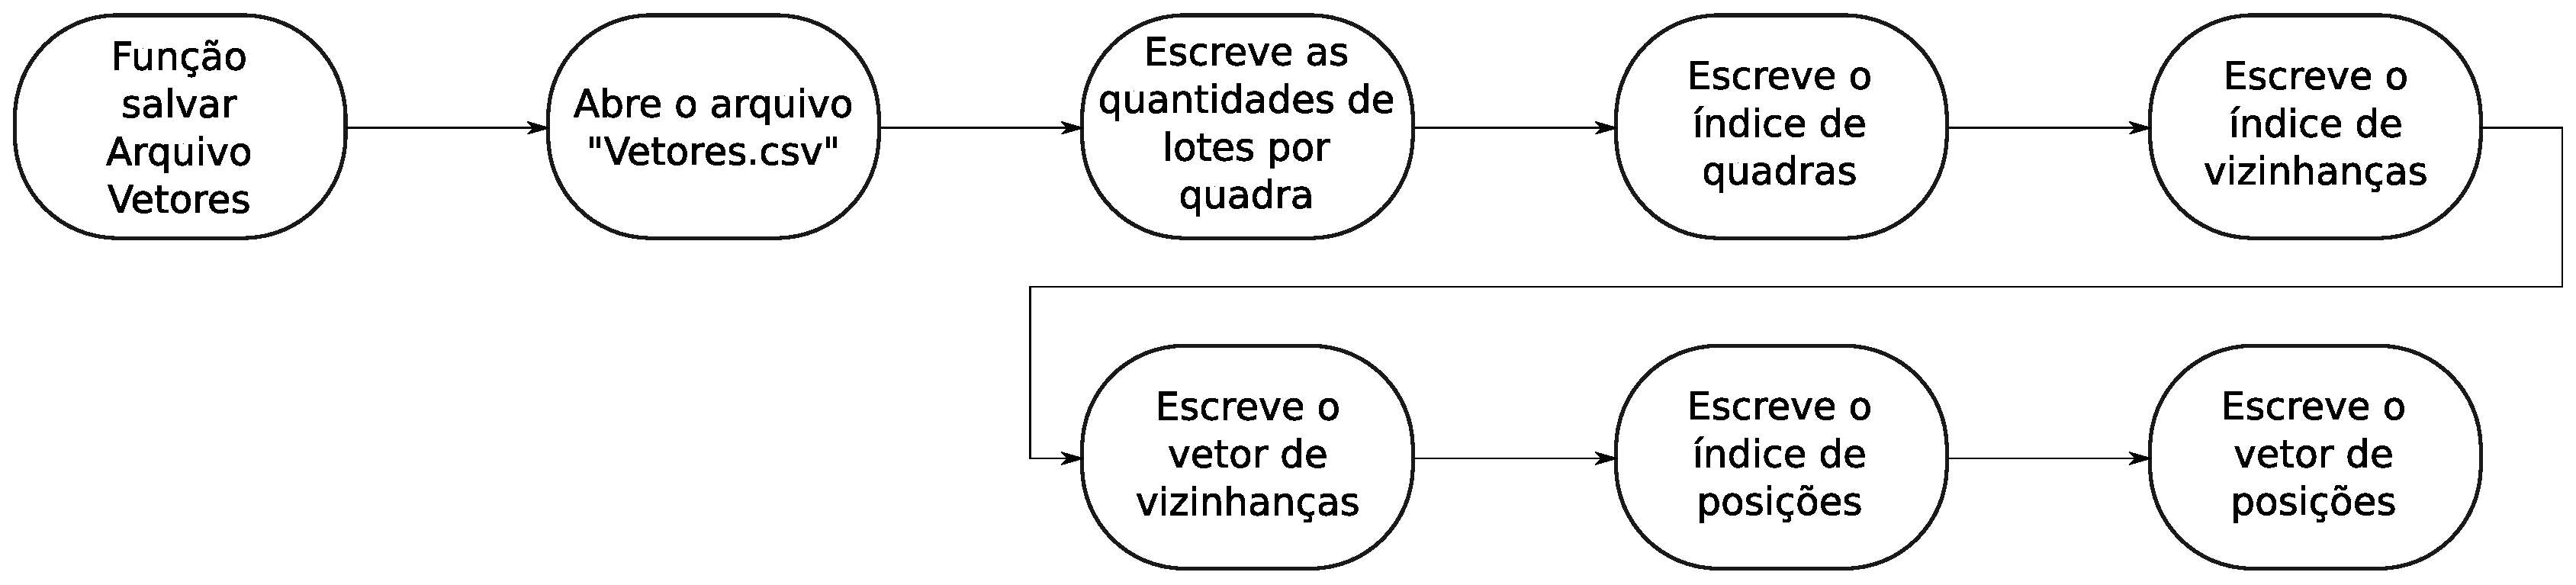
\includegraphics[width=1\textwidth]{Figuras/Simula/Fluxos/salvarArquivoVetores.eps}
  \caption{Função salvarArquivoVetores.}
  \label{fig:salvarArquivoVetores}
\end{figure} 

\newpage

\subsubsection{Função salvarArquivoControles}

O Código \ref{cod:salvarArquivoControles}, Algoritmo \ref{alg:salvarArquivoControles} e Figura \ref{fig:salvarArquivoControles} ilustram a rotina responsável pela escrita do arquivo contendo informações sobre os controles aplicados à população de agentes humanos e percentuais de sazonalidade e quarentena. As informações de controle são escritas no arquivo denominado \textit{"1-CON.csv"}. 

\lstinputlisting[caption=Função salvarArquivoControles, label=cod:salvarArquivoControles, captionpos=b, language=Java]{Codigos/Simula/Fontes/salvarArquivoControles.java}

\begin{algorithm}[H]
   \SetAlgoLined   
   \input{Codigos/Simula/Algoritmos/salvarArquivoControles.txt}
   \caption{\textsc{Função salvarArquivoControles.}}
   \label{alg:salvarArquivoControles}
\end{algorithm}

\begin{figure}[H]
  \centering
  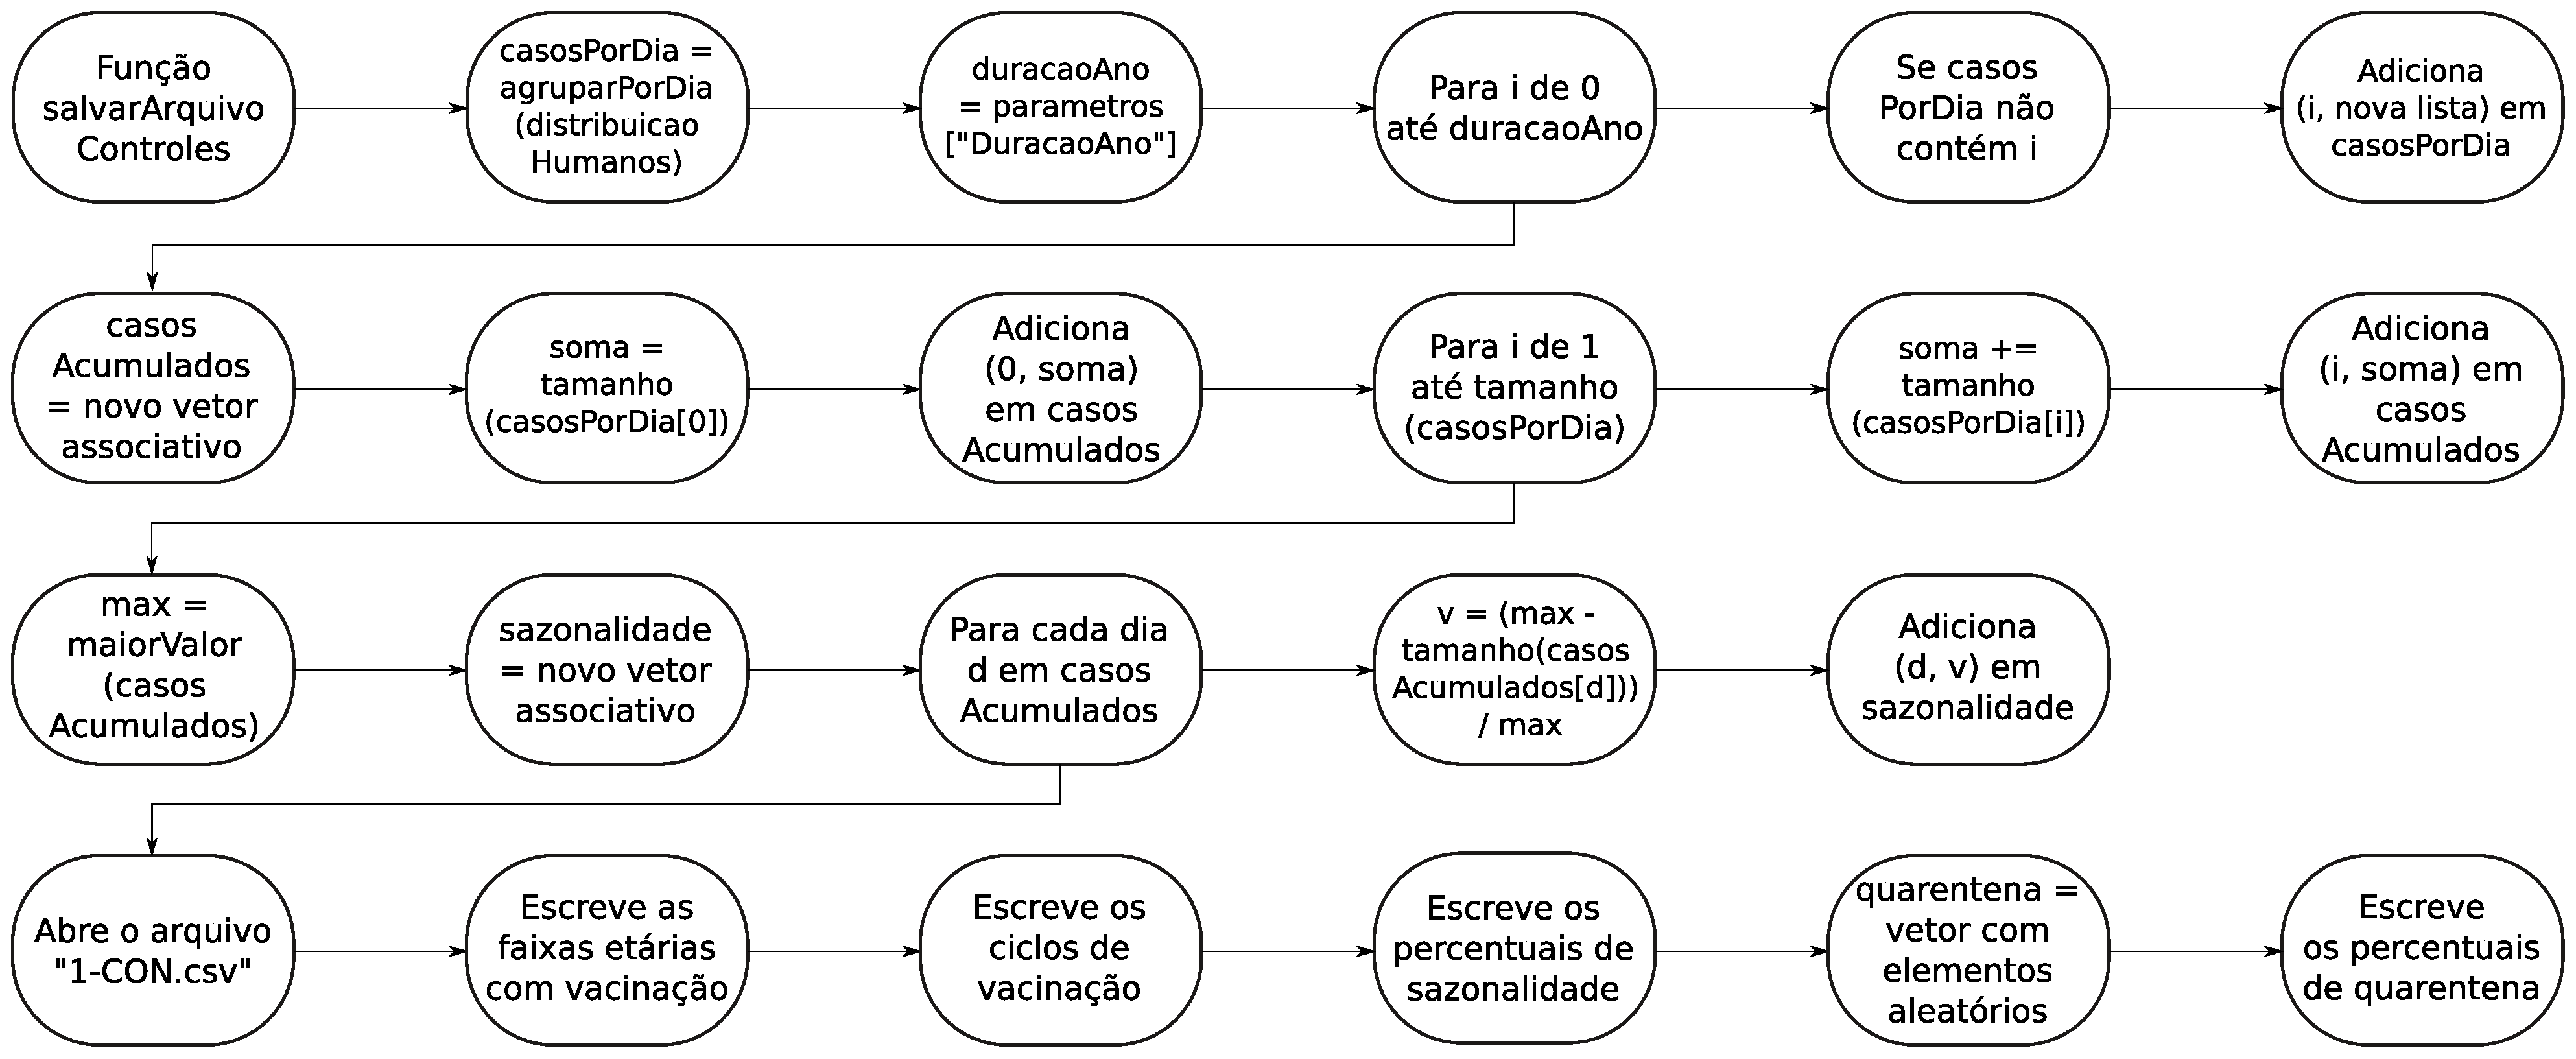
\includegraphics[width=1\textwidth]{Figuras/Simula/Fluxos/salvarArquivoControles.eps}
  \caption{Função salvarArquivoControles.}
  \label{fig:salvarArquivoControles}
\end{figure} 

\newpage

\subsubsection{Função salvarArquivoDistribuicaoHumanos}

O Código \ref{cod:salvarArquivoDistribuicaoHumanos}, Algoritmo \ref{alg:salvarArquivoDistribuicaoHumanos} e Figura \ref{fig:salvarArquivoDistribuicaoHumanos} ilustram a rotina responsável pela geração do arquivo de distribuição dos agentes humanos infectados. Este arquivo é utilizado no processo de inserção de agentes infectados durante o processo de simulação. 

\lstinputlisting[caption=Função salvarArquivoDistribuicaoHumanos, label=cod:salvarArquivoDistribuicaoHumanos, captionpos=b, language=Java]{Codigos/Simula/Fontes/salvarArquivoDistribuicaoHumanos.java}

\begin{algorithm}[H]
   \SetAlgoLined   
   \input{Codigos/Simula/Algoritmos/salvarArquivoDistribuicaoHumanos.txt}
   \caption{\textsc{Função salvarArquivoDistribuicaoHumanos.}}
   \label{alg:salvarArquivoDistribuicaoHumanos}
\end{algorithm}

\begin{figure}[H]
  \centering
  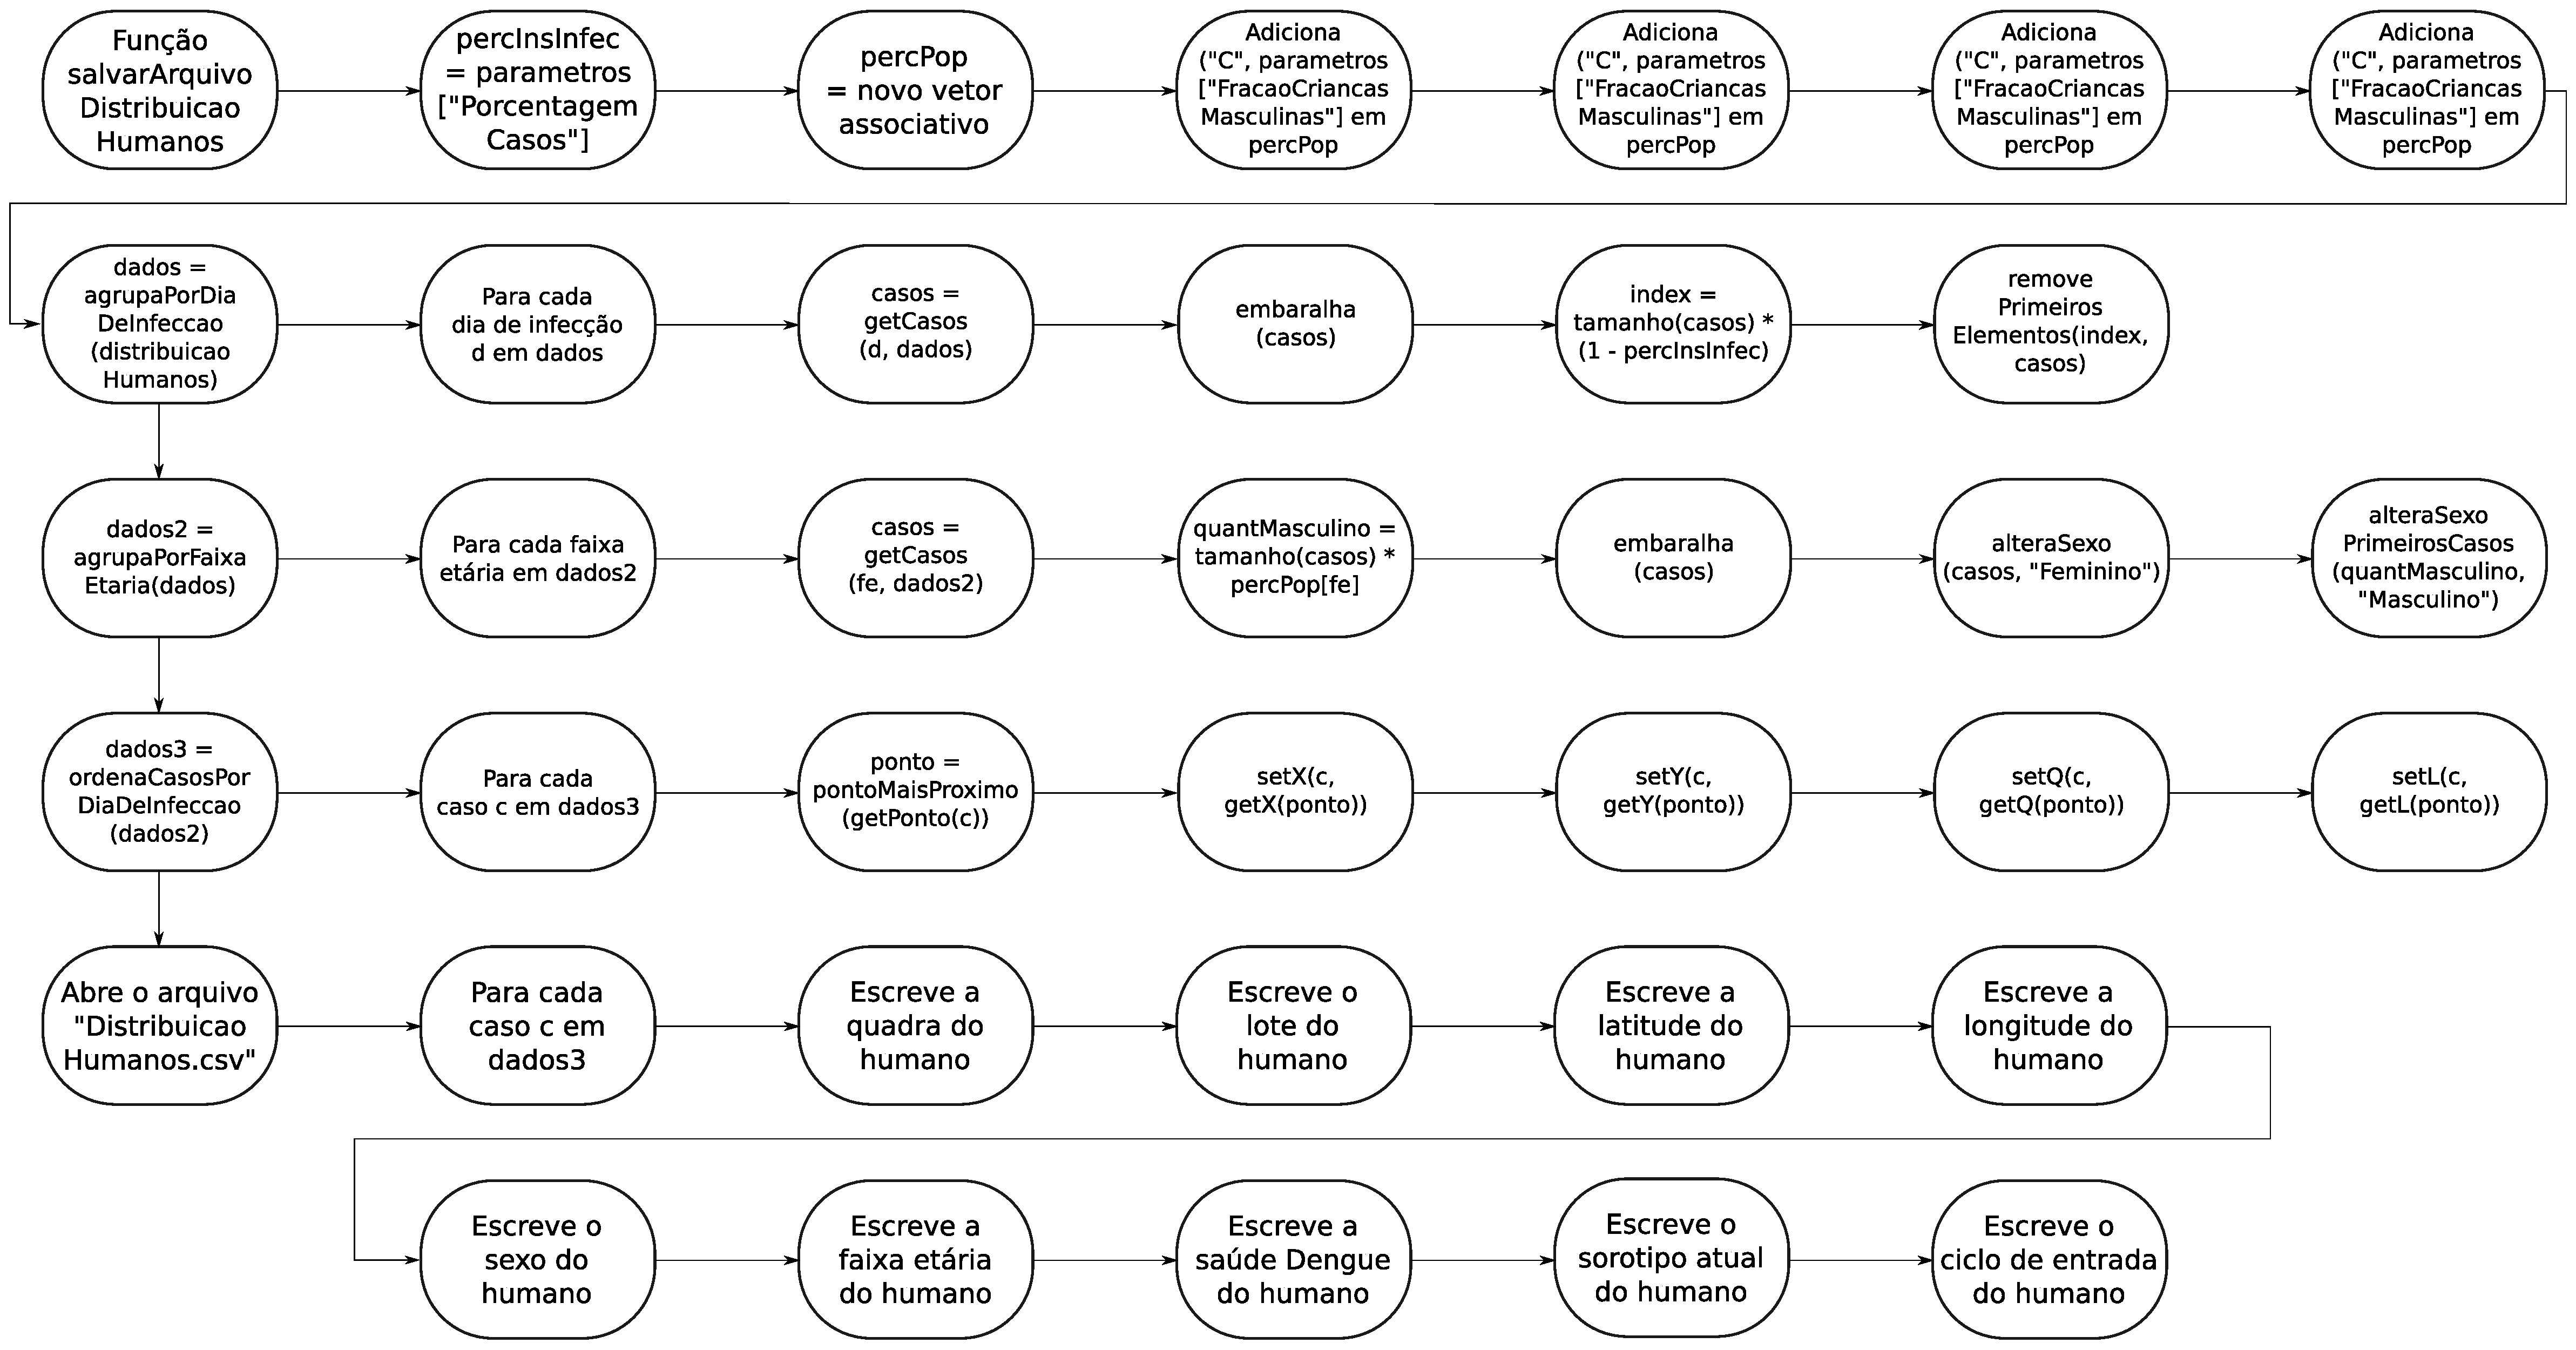
\includegraphics[width=1\textwidth]{Figuras/Simula/Fluxos/salvarArquivoDistribuicaoHumanos.eps}
  \caption{Função salvarArquivoDistribuicaoHumanos.}
  \label{fig:salvarArquivoDistribuicaoHumanos}
\end{figure} 

\newpage
